\documentclass[czech,bachelor]{../../shared/diploma}

% Sablonove baliky
\usepackage[autostyle=true,czech=quotes]{csquotes} % korektni sazba uvozovek, podpora pro balik biblatex
\usepackage[backend=biber, style=iso-numeric, alldates=iso]{biblatex} % bibliografie
\usepackage{dcolumn} % sloupce tabulky s ciselnymi hodnotami
\usepackage{subfig} % makra pro "podobrazky" a "podtabulky"

% Moje baliky
\usepackage{float} % lepsi umistovani obrazku (H)
\usepackage{glossaries} % balik pro praci s odbornymi pojmy
\usepackage{hyperref} % vkladani hypertextovych odkazu
\usepackage{xurl} % zalomeni dlouhych URL
\usepackage{tablefootnote} % poznámky pod tabulkou
\usepackage{color} % barvickyy
\usepackage{array} % schovavani sloupcu v tabulkach

% Pozadovane vstupy pro generovani titulnich stran.
\ThesisAuthor{Barbora Kovalská}
\ThesisSupervisor{Ing. Radoslav Fasuga, Ph.D.}

\CzechThesisTitle{Tvorba herního modelu výpravné evoluční hry}
\EnglishThesisTitle{Creation of the Game Model for the Narrative Evolution Game}

\SubmissionYear{2024}

\ThesisAssignmentFileName{../specification.pdf}

\Acknowledgement{%
Ráda bych na tomto místě poděkovala vedoucímu práce Ing. Radoslavu Fasugovi, Ph.D. za jeho cenné rady a~vedení během tvorby této bakalářské práce. Dále bych chtěla poděkovat kolegům Pavlu Mikulovi, Martinu Korotwitschkovi a~Miroslavu Osobovi za jejich aktivní zapojení, spolupráci a~podněty v~průběhu vývoje. V~neposlední řadě poděkování směřuji svému příteli a~rodině za jejich trpělivost a~podporu během celého studia.
}

\CzechAbstract{%
Hlavním cílem této bakalářské práce je vytvoření a~dokumentace herního systému pro hybridní deskovou hru, která kombinuje fyzické komponenty a~virtuální prostředí. Práce se nejprve zabývá historií deskových her a~studiem klíčových herních mechanik a~analýzou existujících herních modelů. Hlavní část práce se pak věnuje návrhu herního systému, který je založen na principu výpravné evoluční hry. Výsledný herní systém je určen pro hybridní využití fyzických prvků a~digitálního prostředí a~v~kombinaci s~částmi ostatních členů týmu představuje plně realizovanou hru, která poskytuje hráčům bohaté a~dynamické herní zážitky.
}
\CzechKeywords{hybridní desková hra; herní design; rozhodovací pravidla; analýza; evaluace; herní model; týmová spolupráce; herní příručka}

\EnglishAbstract{%
The main goal of this bachelor thesis is to create and document a~gaming system for a~hybrid board game that combines physical components and a~virtual environment. The thesis begins by exploring the history of board games and studying key gaming mechanics, as well as analyzing existing gaming models. The main part of the thesis focuses on designing the gaming system, based on the concept of an narratively evolving game. The resulting gaming system is intended for hybrid use of physical elements and digital environment, and when combined with contributions from other team members, represents a~fully realized game providing players with rich and dynamic gaming experiences.
}
\EnglishKeywords{hybrid board game; game design; decision rules; analysis; evaluation; game model; team collaboration; game manual}

\AddAcronym{API}{Application Programming Interface}
\AddAcronym{CRUD}{Create, Read, Update, Delete}
\AddAcronym{D\&D}{Dungeons \& Dragons}
\AddAcronym{DM}{Dungeon Master}
\AddAcronym{FAQ}{Frequently Asked Questions}
\AddAcronym{JSON}{JavaScript Object Notation}
\AddAcronym{RPG}{Role Playing Game}
\AddAcronym{TTS}{Trails Through Shadows}

\addbibresource{resources/sauce.bib}


% Minted things
\immediate\write18{echo $ROAD > .ROAD.tex}
\immediate\write18{echo $ROAD "nejhorší hack by žožka"}
\input{.ROAD}
\usepackage[outputdir=\ROAD]{minted} %
\setminted{fontsize=\fontsize{9}{11}\selectfont, baselinestretch=1, frame=lines, framesep=8pt, linenos, breaklines}
\renewcommand\listingscaption{Výpis}
\renewcommand\listoflistingscaption{Seznam výpisů zdrojového kódu}

% Command ať nemusím psát celý Dungeons & Dragons;
\newcommand{\dnd}{\textit{D\&D}}

% Uprava hloubky obsahu - pozdeji smazat !
% \setcounter{tocdepth}{2}

% Custom reference
\newcommand{\customref}[2]{\hyperref[#2]{#1~\ref*{#2}}}
\newcommand{\chapterref}[1]{(\hyperref[#1]{Kapitola~\ref*{#1}})} % todo sklonovani jako nullable parametr
\newcommand{\imageref}[1]{(\hyperref[#1]{Obrázek~\ref*{#1}})}
\newcommand{\tableref}[1]{(\hyperref[#1]{Tabulka~\ref*{#1}})}
\newcommand{\glsref}[1]{\textit{\gls{#1}}}
\newcommand{\gameref}[1]{\textit{#1}}
\newcommand{\attr}[1]{(\texttt{#1})}
\newcommand{\devTool}[2]{\textit{#1}\footnote{\href{#2}{#2}}}

% Glossary stuff
\makenoidxglossaries
\loadglsentries{resources/games.tex}

% PlantUML
\newenvironment{plantuml}[1]{\VerbatimOut{#1.puml}}{\endVerbatimOut}
\newcommand{\includeplantuml}[2][]{%
    \IfFileExists{figures/diagrams/out/#2.pdf}{%
        \immediate\write18{if [ figures/diagrams/#2.puml -nt figures/diagrams/out/#2.pdf ]; then java -jar ../../shared/libs/plantuml-1.2024.3.jar -o out -tsvg figures/diagrams/#2.puml; inkscape figures/diagrams/out/#2.svg --export-area-drawing --export-filename=figures/diagrams/out/#2.pdf; rm figures/diagrams/out/#2.svg; fi}
    }{%
        \immediate\write18{java -jar ../../shared/libs/plantuml-1.2024.3.jar -o out -tsvg figures/diagrams/#2.puml; inkscape figures/diagrams/out/#2.svg --export-area-drawing --export-filename=figures/diagrams/out/#2.pdf; rm figures/diagrams/out/#2.svg}
    }
    \includegraphics[#1]{figures/diagrams/out/#2.pdf}
}

% Hide columns in tables
\newcolumntype{H}{>{\setbox0=\hbox\bgroup}c<{\egroup}@{}}


% Zacatek dokumentu
\begin{document}

% Titulni strany
\MakeTitlePages

% Seznam obrazku
\listoffigures
\clearpage

% Seznam tabulek
\listoftables
\clearpage

% Seznam výpisů zdrojového kódu
\addcontentsline{toc}{chapter}{Seznam výpisů zdrojového kódu}
\listoflistings
\clearpage

% Text
\chapter{Úvod}
\label{ch:introduction}


\endinput

\chapter{Historie a~základní pojmy}
\label{chap:theory}

V~této kapitole je ve zkratce popsána historie deskových her, zmíněny některé důležité tituly a~představeny základní pojmy herní teorie a~designu. Veškeré herní tituly, které jsou v~této práci zmíněny, jsou propojeny s~\customref{Přílohou}{chap:game-list}, kde je možné nalézt jejich podrobnější informace.


\section{Historický vývoj}
\label{sec:history}

Deskové hry lidstvo provázejí už překvapivě dlouhou dobu. Ať už sloužily jako zábava, nástroj ke vzdělávání nebo jen jako aktivita umožňující sociální kontakt, vždy byly součástí lidské kultury. Vývoj deskových her odráží vývoj lidské civilizace -- změny v~technologiích, kultuře a~filozofii. Následující kapitoly přibližují historii, kterou si deskové hry v~průběhu času prošly.

\subsection{Počátky}
\label{subsec:beginnings}

Za úplně první deskovou hru by se daly považovat kostky. Ty byly nalezeny v~různých prehistorických nalezištích, což znamená, že lidstvo si s~nimi hrálo dřív, než začalo zanechávat písemné záznamy. Kromě kostek se však našly i~jiné předměty, které byly pravděpodobně používány k~hraní her. Šlo například o~sadu barevných vyřezávaných kamínků, které byly nalezeny v~Turecku, nebo zdobená dřívka z~Mezopotámie. \cite{attia_2018}

Nejstarší nalezená desková hra, historiky pojmenovaná \glsref{royal_game_of_ur}, pochází z~Mezopotámie. Byla objevena v~hrobce krále Ur, který žil před 4500 lety. Hra byla určena pro dva hráče, kteří měli za úkol jako první dopravit své figurky na konec herního pole. Zajímavé také je, že se spolu s~hrou uchovala i~její pravidla, napsaná v~klínovém písmu na destičky. Její věrnou repliku, která je vystavena v~Britském muzeu je možné vidět na \customref{Obrázku}{fig:royal_game_of_ur}. Mezi další hry z~této doby patří například \glsref{senet}, která byla oblíbená v~Egyptě, nebo \glsref{mahjong}, která pochází z~Číny. \cite{british_museum_2021}

\begin{figure}[h]
    \centering
    \includegraphics[width=0.7\textwidth]{figures/images/royal-game-of-ur-british-museum.jpg}
    \caption{Replika hry \textit{The Royal Game of Ur} v~British Museum. \cite{british_museum_2021}}
    \label{fig:royal_game_of_ur}
\end{figure}

Dále by se do této kategorie daly zařadit i~velmi oblíbené \textbf{\glsref{chess}}, které zdánlivě provází lidstvo už od počátků. Jejich historie sahá do roku 400 př. n. l., kdy vznikla keltská hra \glsref{tafl}. Jednalo se o~asymetrickou hru, ve které se jeden hráč snažil utéct se svým králem, začínajícím hru ve středu šachovnice, zatímco druhý hráč se snažil krále chytit. Historici se domnívají, že tato verze byla v~Indii 6. století našeho letopočtu převzata a~pozměněna ve hru \glsref{chaturanga}. Během let její popularita rostla a~rozšířila se do celé Asie a~nakonec i~do Evropy. Do formy, kterou známe dnes, se šachy dostaly právě v~Evropě až v~16. století. \cite{chess_com_2023}

Už takhle brzy je tedy možné zaznamenat dodnes využívané herní principy: herní pole složené z~políček, po kterých se hráči pohybují podle hodů kostkou, a~cíl hry, kterým je dosažení určité pozice na herním poli. \cite{attia_2018}

\subsection{Vývoj deskových her}
\label{subsec:development}

V~období od 18. století se deskové hry stávaly více populárnějšími, s~čímž se také zvedal zájem o~jejich vývoj. Hry byly komplexnější a~jejich tvorba se stala výdělečným odvětvím.

Jako jedna z~prvních vývojářek deskových her je považována Američanka Elizabeth Magie, která v~roce 1903 vytvořila hru \glsref{landlords_game} vyobrazenou na \customref{Obrázku}{fig:landlords-game}. Hra byla zamýšlena jako nástroj k~vzdělávání a~varování proti rizikům land grabbingu -~tedy spekulací s~pozemky. Hráči se v~ní snažili koupit pozemky, stavět na nich domy a~hotely a~tím získávat od ostatních hráčů peníze. V~roce 1935 Magie prodala patent na hru společnosti \textit{Parker Brothers} za 500 dolarů. Ti hru přejmenovali na \textbf{\glsref{monopoly}} a~začali ji prodávat, což se ukázalo být velmi úspěšné. \cite{attia_2018}

\begin{figure}[h]
    \centering
    \includegraphics[width=0.4\textwidth]{figures/images/landlords-game.png}
    \caption{Hra \textit{The Landlord's Game} od Elizabeth Magie. \cite{attia_2018}}
    \label{fig:landlords-game}
\end{figure}

V~Německu se deskové hry rozrostly tak moc, že se zde okolo nich vytvořila vlastní kultura. V~roce 1978 byla založena společnost \textit{Spiel des Jahres}, která každý rok uděluje cenu pro nejlepší hru roku. Tato cena se stala velmi prestižní, zvýšila zájem o~deskové hry po celém světě a~pomohla k~úspěchu mnohým hrám jako \glsref{catan} nebo \glsref{dixit}. \cite{attia_2018}

\subsection{Moderní směr}
\label{subsec:modern}

Kvůli vzniku a~úspěchu spousty dalších her, například \glsref{carcassonne}, \glsref{ticket_to_ride} nebo \glsref{risk}, čím dál více lidí chtělo vyvíjet hru vlastní. V~tomto jim pomohl jeden z~dalších milníků -~vznik projektu Kickstarter. Tato platforma umožňuje vývojářům prezentovat své nápady a~získat na ně finanční podporu od lidí, kteří by je chtěli vidět na trhu. \cite{attia_2018}

Díky tomu deskové hry prošly revolucí, neboť nyní zde byla možnost propagovat hru přímo hráčům, kteří by ji chtěli hrát. Velmi úspěšné projekty jako \glsref{exploding_kittens} nebo \glsref{gloomhaven} získaly na platformě Kickstarter miliony dolarů. Také zde začaly vznikat deskové implementace existujících videoherních titulů, jako například \glsref{darkest_dungeon}, \glsref{witcher} nebo \glsref{dark_souls}. \cite{kickstarter}

Nesmí být opomenut ani gigant mezi deskovými hrami, který přinesl revoluci v~herním designu -~\textbf{\glsref{dnd}}. Tato hra, vytvořená Gary Gygaxem a~Davidem Arnesonem, byla první stolní hrou, která se zaměřovala na příběh a~roleplay, neboli hraní určité role v~rámci herního světa. Hráči si v~ní vytvářeli své postavy a~procházeli s~nimi dobrodružstvím, které jim připravoval tzv. \textit{Dungeon Master} -~hráč, který hru řídil a~vytvářel pro ostatní dobrodruhy příběh. Tento nápad byl tak úspěšný, že vytvořil celý žánr -~\textit{tabletop RPGs} -~a~inspiroval spoustu dalších her, jak deskových, tak videoherních. \cite{dnd_beyond_2023}

V~moderních hrách je možné pozorovat, že se stále více zaměřují na roleplay a~příběh a~hlouběji implementují \textit{RPG} prvky, jako jsou vyvíjející se postavy, dialogy nebo větší důraz na spolupráci mezi hráči. I~herní mechanismy se stávají více komplexními a~vývojáři se nebojí experimentovat s~novými nápady. Hry začínají být i~obsáhlejší, což se projevuje v~delší době hraní, větší složitosti pravidel a~větším množství fyzických komponent.


\section{Definice pojmu desková a~stolní hra}
\label{subsec:boardgame_definition}

V~této oblasti herního designu se vyskytují dva základní pojmy: \textit{desková hra} a~\textit{stolní hra}. Tyto termíny jsou často užívány jako vzájemně zaměnitelné, přestože nesou odlišné významy. V~této kapitole jsou tyto pojmy podrobněji rozebrány.

\textbf{Desková hra} (board game) je obvykle hra, jejíž hlavní a~neoddělitelnou součástí je herní deska. Samotné provedení desky se může lišit, může se jednat o~klasickou čtvercovou desku, nebo o~jiný tvar, jako například kruhovou, hexagonální nebo jinou. Deska může být také rozdělena na políčka, která mohou mít různé vlastnosti, například barvu, číslo nebo symbol. Hra může mít také další komponenty, jako jsou karty, kostky, figurky, žetony, atd. Herní systém většinou bývá intuitivní a~jednoduchý, snažící se zaměřit na širší publikum hráčů. Herní mechaniky se často soustředí na desku a~ostatní fyzické komponenty a~neobsahují velkou míru abstrakce. Do této kategorie patří například \glsref{monopoly}, \glsref{catan} nebo \glsref{carcassonne}. \cite{board_game_supply_2023}

\textbf{Stolní hra} (tabletop game) je obecnější termín, který zahrnuje všechny hry, které se hrají na stole. To znamená, že do této kategorie můžeme zařadit i~hry, které nemají herní desku, jako například karetní hry, hry s~kostkami, nebo hry, které se hrají pouze s~papírem a~tužkou. I~když jsou komponenty jejich důležitou součástí, některé stolní hry si dovolují vyšší míru abstrakce herních systémů, což jim dává větší možnosti hloubky na úkor odcizení některých skupin hráčů. Toto můžeme pozorovat například u~prosperujícího žánru \textit{RPG} her, kam můžeme zařadit \glsref{forgotten_waters}, \glsref{gloomhaven} nebo i~výše zmíněné \glsref{dnd}. \cite{board_game_supply_2023}

Pro účely této práce bude pozornost věnována především deskovým hrám, přičemž se bude usilovat o~zahrnutí některých prvků stolních her, jež by mohly být pro návrh užitečné.

\chapter{Teorie herního designu}
\label{chap:design}

V této kapitole si popíšeme základní pojmy herní teorie a designu, které nám poslouží jako základ pro náš vlastní návrh. \cite{building_blocks_of_tabletop_design_2022}


%%% section: Structure %%%

\section{Herní struktura}
\label{sec:basics}

Herní struktura je základním stavebním kamenem každé hry. Jedná se o sadu pravidel, která určují, jak se hraje, co mohou hráči dělat a jakým způsobem se hra vyhrává. Typy struktur se liší podle jejich přístupu k herním systémům a mechanikám. 

\subsection{Kompetetivní hry}
\label{subsec:competitive}

Kompetetivní hry tvoří velkou část trhu s deskovými hrami. V těchto hrách se hráči snaží porazit ostatní a dosáhnout vítězství. Tyto hry můžou být symetrické, kdy všichni hráči začínají se stejnou nebo alespoň podobnou silou, nebo asymetrické, kdy mají hráči různé schopnosti a cíle. Častým problémem bývá vybalancovat hru tak, aby byla zábavná pro všechny hráče, a to i přesto, že se může stát, že jeden hráč bude mít výhodu. Dále se často stává, že hra skončí remízou. V takovém případě se může o vítězi rozhodnout buď pomocí nějakých dodatečných pravidel, nebo může skončit sdíleným vítězstvím.

Příklady: \textit{Monopoly}, \textit{Carcassonne}, \textit{Šachy}, \textit{Race for the Galaxy}

\subsection{Kooperativní hry}
\label{subsec:cooperative}

Naopak kooperativní hry se snaží hráče spojit proti společnému nepříteli nebo problému. Hráči spolupracují na dosažení cíle, který je obvykle nějakým způsobem předem daný. Velkou výhodou toho typu her je to, že odstraňují překážky, které by lidem bránily si tento typ her zahrát. Když jsou hráči spolu ve stejném týmu, dokáží vyrovnat jejich schopnosti a zkušenosti, což může novým hráčům pomoci se do hry dostat.

Kooperativní hry se dají dále rozdělovat podle různých kritérií. Například některé mohou hráče spojit v boji proti oponentovi ve formě umělé inteligence nebo sady algoritmů, zatímco jiné dávají týmu za úkol vyřešit hádanku a nemají žádného protivníka. Dalším kritériem může být, jestli hra má skryté informace, nebo jestli jsou všechny informace sdílené. Sdílení zdrojů, způsob komunikace a způsob, jakým se hra vyhrává, jsou dalšími faktory, které mohou kooperativní hru ovlivnit.

Příklady: \textit{Pandemic}, \textit{Arkham Horror}, \textit{Gloomhaven}, \textit{Na vlnách neznáma}


\subsection{Hry se scénářem}
\label{subsec:scenario}

Tento typ her se často zaměřuje především na příběh, historickou tematiku a RPG elementy. Průběh hrou se skládá z jednotlivých epizod, které můžou být předem naplánované a navázané na sebe. Tento systém se často používá v tzv. \textit{dungeon crawlerech}, kde hráči prochází jeden dungeon za druhým. S tímto formátem je jednoduché vyměnit mapu, typy nepřátel nebo příběhové zabarvení a hráči mohou zažít více dobrodružství bez toho, aby se museli učit nová pravidla. Taky je to jednoduchý způsob jak nastavit obtížnost hry, protože každý scénář může být jiný.

Příklady: \textit{Osadníci z Katanu}, \textit{Gloomhaven}, \textit{Pathfinder}

\subsection{Legacy hry}
\label{subsec:legacy}

Legacy hry jsou speciální typ her, který se vyznačuje nenávratnými změnami, které hráči během hraní páchají na herních komponentách. Jde o změny fyzického rázu, jako je psaní na herní desku, trhání karet nebo lepení nálepek. Tyto změny mohou být způsobeny výsledkem hry, nebo mohou být součástí příběhu. Tento typ her se často zaměřuje na příběh a vývoj postav, a proto mají velmi blízko k RPG žánru. Kampaně v nich mohou trvat i několik měsíců či let, rozdělených do jednotlivých několikahodinových sezení. Jedná se o relativně nový fenomén, který se však v posledních letech začal rozšiřovat a získal si své publikum.

Příklady: \textit{Risk Legacy}, \textit{Harry Potter: Hogwarts Battle}, \textit{Gloomhaven}


%%% section: Turns %%%

\section{Pořadí a struktura tahů}
\label{sec:turns}

Se zavedením struktury přichází potřeba rozhodovat, kdy hráči mohou konat různé akce nebo kroky. Odsud vznikla myšlenka \textbf{tahu} - jednotky času, během které mohou hráči se hrou interagovat. Více tahů pak tvoří jedno \textbf{kolo}, přičemž běžné hry se skládají z několika takovýchto kol. V některých titulech se kola navíc rozdělují do několika \textbf{fází}, které většinou rozdělují akce do různých typů, čímž umožňují ještě větší stukturovanost herního kola. Tato pravidla se však mohou lišit podle typu hry, a proto si zde přiblížíme několik základních typů struktury tahů.

\subsection{Kolo s pevným pořadím}
\label{subsec:fixed_order}

Jedná se o nejzákladnější typ struktury kola, kdy se pořadí hráčů určí jednou na začátku hry a od té doby zůstává neměnné. Obvykle se nějakým způsobem vybere první hráč a dál tahy pokračují podél stolu ve směru nebo proti směru hodinových ručiček (například v klasické karetní hře \textit{Prší}). Tento typ struktury je velmi jednoduchý a intuitivní, ale může být nevýhodný pro hry, kde je výhoda mít první tah, nebo chceme zajistit, aby všichni hráči měli stejný počet tahů. Toto se dá řešit zvýhodněním odstaních hráčů jinými způsoby, například herními bonusy (mana navíc pro druhého hráče v \textit{Hearthstonu}), nebo tím, že budeme monitorovat, který hráč začínal, a poslední kolo se vždy dojede až k němu, i kdyby hra byla ukončena v průběhu kola (jako v \textit{Through the Ages}, kde všichni dojedou celé kolo po tom, co jeden hráč zvítězí).

\subsection{Kolo s pořadím podle statistik}
\label{subsec:stat_order}

Tento typ struktury kola se snaží vyrovnat výhody a nevýhody, které mohou vzniknout z pevného pořadí. Pořadí se v tomto případě mění podle nějakého skóre, které se během hry mění. Určující statistikou může být například počet bodů, které hráči mají (tokeny populace v \textit{Civilizaci}), nebo nějaké pevnější statistiky spojené se samotnými postavami. Tento systém se často používá v RPG hrách, kde se pořadí může měnit podle iniciativy postav (klasická iniciativa v \textit{D\&D}), nebo ve hrách, kde se pořadí mění podle toho, jak dobře nebo špatně se hráči daří (znevýhodnění nejlepších hráčů ve \textit{Vysokém napětí}). Hra pak dokáže být dynamičtější a aktivně reagovat na změny, což přináší nové strategické možnosti a větší zapojení hráčů.

\subsection{Kolo s pořadím určeném v reálném čase}
\label{subsec:realtime_order}

Další zajímavou možností určení pořadí je nechat hráčům volnou ruku, často omezenou nějakým časovým limitem. Je pak na rychlosti samotných hráčů, jak rychle dokážou reagovat na situaci a provést svůj tah. Silnou stránkou tohoto systému je to, že hra může být mnohem rychlejší a dynamická a často s sebou přináší vyšší úroveň soutěživosti (například u hry \textit{Dobble}). Nevýhodou je to, že může být pro některé hráče stresující a může být obtížné udržet přehled o tom, co se děje. Také se designer musí více rozmyslet, jak řešit chyby hráčů a také podvádění, které v tomto zmatku bývá častější.

\subsection{Kolo s náhodným pořadím}
\label{subsec:random_order}
% TODO - najít hru, která tohle používá

Náhodný výběr figurek nebo žetonů reprezentujících jednotlivé hráče, často losované z pytlíku nebo balíčku, je skvělý způsob, jak udělat hru méně předvídatelnou. Bohužel s sebou nese i snížené možnosti strategie ze strany hráčů, takže se hodí spíše pro hry, které nemají s náhodou problém a snaží se být spíše zábavné a chaotické. V opačném případě se musí zavést nějaké doplňkové mechanismy, které hráčům umožní reagovat na náhodu a otočit ji ve svůj prospěch.

\subsection{Kolo se současným výběrem akcí}
\label{subsec:action_selection_order}

Posledním typem struktury kola, který si zde přiblížíme, je kolo, kde hráči vybírají akce současně, často v tajnosti. Když jsou všichni připraveni nebo po uplynutí nějakého určeného času, se všechny akce odhalí najednou a provedou se (v \textit{Gloomhavenu} si hráči nejprve zvolí své akce, ale provést je mohou, až když na ně přijde řada). Často je tady třeba také druhotná mechanika pro určení pořadí, ve kterém se akce vyhodnotí (například v \textit{Race for the Galaxy}, kde si hráči nejprve zvolí fáze, které chtějí hrát, a pak si v tajnosti zvolí akce, které se pak vyhodnotí v pořadí vybraných fází). Tajné vybírání akcí je vhodné pro hry, které dávají důraz na strategii a odhadování akcí soupeřů.


%%% section: Actions %%%

\section{Akce}
\label{sec:actions}

\subsection{Akční body}
\label{subsec:action_points}

\subsection{Omezený výběr akcí}
\label{subsec:limited_actions}

\subsection{Pálení akcí}
\label{subsec:burning_actions}

\subsection{Výběr příběhu}
\label{subsec:story_choice}

\subsection{Rozhodnutí akce}
\label{subsec:action_resolution}


%%% section: Movement %%%

\section{Pohyb po herním poli}
\label{sec:movement}

\subsection{Rozdělení pole}
\label{subsec:tessellation}

\subsection{Pohyb podle hodu kostkou}
\label{subsec:roll_movement}

\subsection{Pohyb podle ceny}
\label{subsec:cost_movement}

\subsection{Odhalování terénu}
\label{subsec:map_reveal}

\subsection{Více map}
\label{subsec:multiple_maps}


%%% section: End %%%

\section{Konec hry}
\label{sec:end}

\subsection{Body vítězství}
\label{subsec:victory_points}

\subsection{Závod}
\label{subsec:race}

\subsection{Vyčerpání zdrojů}
\label{subsubsec:resource_depletion}

\subsection{Kooperativní cíle}
\label{subsec:cooperative_goals}
\chapter{Analýza existujících her}
\label{chap:game_analysis}

Tato kapitola se zaměřuje na analýzu několika existujících deskových her, které poslouží jako inspirace pro vlastní návrh modelové hry. Rozebrány budou klady i zápory těchto her, co je dělá zajímavými, co je na nich dobré a co by naopak bylo třeba změnit. Analýza se bude zaměřovat především na herní principy, které byly uvedeny v předchozí kapitole \chapterref{chap:game_design}.


%%% Forgotten Waters %%%

\section{Na vlnách neznáma}
\label{sec:forgotten_waters}

\glsref{forgotten_waters} (anglicky \textit{Forgotten Waters}) je kooperativní desková hra pro 3 až 7 hráčů, kterou vydalo v roce 2020 vydavatelství Plaid Hat Games. Hra je zasazena do fantasy světa, kde hráči přebírají role pirátů, jejichž úkolem je spolupracovat, aby úspěšně splnili sen jejich kapitána. Každá z postav má však své vlastní cíle, které jsou reprezentovány vývojem postavy a jejími schopnostmi. Důležitou součástí hry je webová aplikace, která poskytuje hudební a zvukové efekty, včetně hlasového vyprávění, které hráče provází příběhem a vytváří tak atmosféru hry. \cite{forgotten_waters}


\subsection{Herní systém}
\label{subsec:fw_gameplay}

Z pohledu herní struktury tato hra jednoznačně spadá do kategorie kooperativních her \chapterref{subsec:structure_cooperative}, je však obohacena i o prvky scénářových \chapterref{subsec:structure_scenario} a legacy her \chapterref{subsec:structure_legacy}. Před samotnou hrou si hráči vyberou, pod kterým kapitánem budou sloužit jako posádka, což je v podstatě abstrakce nad pouhým vybráním herní kampaně, která obsahuje předpřipravený scénář, včetně herní mapy a příběhu, kterým budou hráči procházet. Samotná hra pak spočívá v cestování mezi lokacemi a potýkání se s událostmi, které tyto lokace nesou. Kampaň je rozdělena do několika částí, mezi kterými jsou hráči vybídnuti, aby si hru uložili a pokračovali v ní později. Jednotlivé části mohou trvat několik hodin, pokud však hráči chtějí, kampaň jde odehrát během jednoho dlouhého sezení. Herní komponenty se hrou však přímo neznehodnocují, s jedním balením je možné odehrát libovolný počet kampaní.

Lokace se ve hře vybírají pomocí pohybu lodi po mapě tvořené hexagony. Podle scénáře jsou některé hexagony předem určené, jiné jsou prázdné a když na ně hráči stoupnou, umístí místo nich náhodně vylosovanou lokaci. Herní pole je tedy rozděleno dvoudimenzionálně a mění se dynamicky \chapterref{subsec:map_reveal} podle postupu posádky. Pohyb lodi je ovlivněn hodem hráče, který si vybral, že ji bude toto kolo řídit. Podle jeho úspěšnosti se loď posune u určitý počet polí, pohyb je tedy náhodný \chapterref{subsec:movement_roll_movement} s přidanými modifikátory.

V rámci lokace je hráčům představeno několik možností, které si může vybrat buď několik lidí, nebo jsou přístupné pouze prvnímu z nich \chapterref{subsec:actions_limited_actions}. Některé z nich jsou také povinné - musí si je vybrat alespoň jeden hráč. Tyto možnosti jsou reprezentovány jako vytištěný seznam akcí na stránce knihy, která je součástí balení. Výběr akcí probíhá v pořadí iniciativy, která je reprezentovaná stupnicí věhlasu, jde tedy pořadí podle jisté statistiky \chapterref{subsec:turns_stat_order}. Samotné vyhodnocování probíhá v pořadí od první akce po poslední tak, jak jsou na stránce vytištěny.

Co se týče konce hry, ten je určený předem připraveným scénářem. Každá část končí nějakou událostí, která se vyvolá po dokončení lokace. Po dokončení všech částí hry je dokončen i příběh a následuje příběhový epilog, vyhodnocený podle toho, jak se hráči během hry chovali. Jde tedy o příklad ukončení na základě splnění kooperativního cíle \chapterref{subsec:end_cooperative_goals}. Na závěr hry však ještě probíhá vyhodnocení příběhu jednotlivých postav, které v průběhu hry získávají body souhvězdí, které následně určují, jakým způsobem se příběh postavy vyvine. Jedná se tedy o ukázku konce hry na podle bodů vítězství \chapterref{subsec:end_victory_points}.


\subsection{Fyzické komponenty}
\label{subsec:fw_components}

\glsref{forgotten_waters} svůj herní systém podporuje několika fyzickými komponenty, které jsou součástí balení hry. Ty nejdůležitější z nich jsou přiblíženy níže.

\subsubsection*{Herní deska}
\label{subsubsec:fw_comp_board_and_book}

Herní deska je tvořena hexagonálním polem, které reprezentuje moře, po kterém se hráči pohybují. Na tuto prázdnou šablonu se umisťují hexagonální žetony navigace, které představují místa, kterými hráči proplouvají. Když hráči plují přes prázdné pole, náhodně vylosují žeton, který na toto pole umístí, což dodává hře pocit, že v ní opravdu prozkoumávají neznámé moře. Jednotlivé žetony navigace mají své vlastní identifikační číslo, které přes aplikaci odkáže hráče na příslušnou stránku v knize lokací.

Kniha lokací je příručka, která obsahuje všechny lokace, které mohou hráči navštívit. Každá lokace má svou vlastní stránku, na které je popsána, včetně možností, které na ní hráči mají. Na levé straně jsou vždy vytištěné jednotlivé akce, na které si hráči během kola postaví své figurky a dále s těmito akcemi pracují. Na pravé straně je vytištěný tematický obrázek, který hře dodává atmosféru.

\subsubsection*{Karty}
\label{subsubsec:fw_comp_cards}

Většina ve hře karet reprezentuje předměty, které mohou hráči získat a použít. Dělí se na poklady, které hráči získávají různými způsoby během hry, a příběhové karty, které se vztahují k příběhu postav. Karty přinášejí bonusy ke schopnostem, které postavy mohou využít, a také mohou nést složitější bonusy, které jsou ve zkratce popsané na kartě. Jedná se o jednoduchý způsob, jak hráčům umožnit jedinečný vývoj jejich postav, který je zároveň snadno zpřístupněný a přehledný.

\subsubsection*{Postavy a role}
\label{subsubsec:fw_comp_roles}

Jako posádka lodi si hráči před začátkem hry rozdělí role, o jejichž povinnosti se musí postarat. Spolu se svou rolí dostanou i list nebo desku, která slouží jako počítadlo pro různé statistiky, které budou hlídat. Jedná se o následující role:

\begin{itemize}
    \item \textbf{Lodní písař}: Stará se o lodní deník.
    \item \textbf{Kormidelník}: Hlídá věhlas, který určuje iniciativu při výběru akcí.
    \item \textbf{První důstojník}: Hlídá nespokojenost a počet členů posádky.
    \item \textbf{Bocman}: Kontroluje stav trupu - pokud se loď potopí, hra končí.
    \item \textbf{Bednář}: Hlídá lodní zásoby.
    \item \textbf{Dělostřelec}: Obsluhuje lodní děla, která se využívají především v soubojích.
    \item \textbf{Pozorovatel}: Hlídá průběh příběhu.
\end{itemize}

Pomocí takovéhoto rozdělení rolí mezi hráče je zajištěno, že se všichni hráči budou muset podílet na řízení lodi, a zároveň se také zamezí tomu, aby se některé činnosti opakovaly.

Samotné postavy také mají své vlastní deníky. Tyto deníky slouží jako záznamník pro vývoj postavy, který je reprezentován body souhvězdí, které postava získává během hry. Po konci příběhu se podle těchto bodů vyhodnotí, jaký osud postavu potkal. Kromě těchto příběhů a jejich potenciálu na získávání schopností různé úrovně se však postavy moc neliší.

\subsubsection*{Kostky}
\label{subsubsec:fw_comp_dice}

Pro vyhodnocování úspěšnosti akcí se ve hře používají dvanáctistěnné kostky, které se hází vždy, když je třeba určit výsledek zkoušky dovednosti. Když si hráč háže například na sílu, k výsledku hodu kostkou přičte svou vlastní hodnotu síly a případně bonusy, které mohl získat z karet. Výsledek pak porovná s obtížností úkolu, kterou určuje scénář.

Zpestření hodů zajišťují speciální žetony, které upravují výsledek hodu. Jedná se o žetony neštěstí, při kterých si hráč musí hodit znovu a počítat si horší výsledek, a žetony přehození, které naopak umožňují ze dvou výsledků počítat ten lepší. 

\subsubsection*{Figurky}
\label{subsubsec:fw_comp_figures}

\glsref{forgotten_waters} nepoužívá přímo figurky, ale volí levnější variantu - tzv. standees, ilustrace vytištěné na kartonu, které se postaví do plastových stojanů. Tyto standees reprezentují jak postavy v rámci lokace, tak i samotnou loď na herním plánu. Jednoduchost tohoto způsobu umožňuje snadnou reprezentaci postav a zároveň snižuje náklady na výrobu hry.


\subsection{Podpůrné aplikace}
\label{subsec:fw_apps}

Hlavní funkcionalitu, kterou aplikace přináší, je průvodce příběhem. Při vstupu si hráči zvolí kampaň, kterou chtějí hrát, načež jim aplikace přehraje úvodní dialog a pokud je to potřeba, krok po kroku jim ukáže, jak si mají herní desku a ostatní komponenty připravit. Dále aplikace slouží jako knihovna informací. Každý záznam, který hráčům ukazuje, má svůj třímístný kód, pomocí jehož hráči mohou na záznamy přistupovat. Tento přístup poskytuje vývojářům velkou flexibilitu v tom, odkud mohou hráči kódy získávat. Může jít o pouhé uvedení lokace (jak již bylo výše zmíněno, každá lokace má svůj odpovídající kód), krátkou anekdotu po získání nového předmětu nebo i o příběhový výsledek nějakého rozhodnutí. Jako vedlejší funkci aplikace také přináší hudební a zvukové efekty, které hru doplňují a vytváří kýženou atmosféru. \cite{fw_crossroads_app}

Nově také vznikla oficiální webová aplikace, která umožňuje hru hrát plně online. Na stránkách je možné si založit herní místnost, do které se mohou připojit ostatní hráči. Během hry jsou pak digitalizovány všechny komponenty, které jsou potřeba k hraní, včetně herní desky, knihy lokací, karet a počítadel pro jednotlivé role. \cite{fw_remote_app}

\subsection{Herní pravidla}
\label{subsec:fw_rules}

Pravidla hry \glsref{forgotten_waters} jsou přiložena jako součást balení, jsou však přístupná i v digitální formě na stránkách vydavatele. Hned ze začátku jsou hráči seznámeni s důležitostí webové aplikace a je jim předložen odkaz, přes který se na ni dostanou. Následně je ve zkratce uveden a shrnut veškerý herní materiál, který je v balení obsažen, a složitější komponenty jsou vyobrazeny nákresem s popisky klíčových částí.

Hlavní část pravidel je věnována popisu postupu na přípravu hry a průběhu jednotlivých kroků. Příprava je rozepsána do očíslovaných kroků a doplněna o ilustrace, které hráčům usnadňují orientaci. Následně je hráčům vysvětleno, jak je rozděleno kolo a jak fungují akce v něm. Dále jsou také přiblíženy jednotlivé postavy, jejich dovednosti a zkoušky, které se k nim vztahují. Na závěr jsou hráči seznámeni s tím, jak může hra skončit, ať už pozitivně či negativně, a jak se hra ukládá, pokud se rozhodnou ji hrát v oddělených sezeních. Jako zajímavý bonus na konci pravidel je přiložen generátor pirátských jmen, který hráčům pomocí dvou kostek umožní vygenerovat si jméno pro svou postavu.


%%% Dungeons & Dragons %%%

\section{Dungeons \& Dragons}
\label{sec:dungeons_and_dragons}

Obrovský vliv, který měla revoluční RPG hra \glsref{dnd} na vývoj stolních her, už byl zmíněn výše. Tato hra je však také zdrojem inspirace pro mnoho deskových her, které se snaží přenést některé z jejích prvků do stolního prostředí, a rozšířit tím svou potenciální hráčskou základnu. Tato sekce se zaměřuje na analýzu prvků, které byly převzaty z \dnd{} do jiných her. Oproti jiným hrám, které jsou v této práci rozebrané, je však \dnd{} mnohem komplexnější a množství jeho herních mechanik je také mnohem větší, proto se tato sekce bude držet spíše herních systémů a mechanik, které jsou popsány ve výše zmíněné kapitole \textit{\nameref{chap:game_design}}.


\subsection{Herní systém}
\label{subsec:dnd_gameplay}

Prvně je třeba zmínit, že \dnd{} se nedrží klasické symetrické struktury, kterou většina stolních her využívá. Hra je založena na asymetrickém systému, kde jeden z hráčů, označovaný jako \textit{Dungeon Master} (DM) nebo vypravěč, má na starosti vytváření a řízení celého světa, včetně všech postav, které v něm žijí. Ostatní hráči, v tomto světě následně hrají své vlastní postavy a dělají za ně rozhodnutí, stěžejní částí herního zážitku je tedy \textit{roleplay}. Tento systém je základem pro všechny ostatní mechaniky, které jsou v této hře používány. Z tohoto popisu se může zdát, že hráči a DM soupeří o jakousi výhru, ve skutečnosti však spolupracují na vytváření příběhu, který je pro všechny zúčastněné zábavný. Tatu skutečnost z \dnd{} dělá nejen pouhou stolní hru, ale prostředek pro kooperativní vyprávění příběhů.

Svou strukturou je \dnd{} ukázkovým příkladem legacy hry \chapterref{subsec:structure_legacy}, neboť běžná kampaň může trvat až roky a z pohledu ničení herních komponent se tato charakteristika odvíjí od konkrétní kampaně a také kreativity DM a ostatních hráčů. Je zřejmý také strukturální vliv scénáře \chapterref{subsec:structure_scenario} -- pro hráče je přístupná spousta předpřipravených scénářů a kampaní, kterými se DM může řídit, ať už jde o oficiální příběh od vývojářů nebo o neoficiální práci některého z mnoha fanoušků, tvořící pro hru další obsah. Hráči se však příběhu nemusí držet, pokud nechtějí, neboť volnost herních mechanismů dává velkou flexibilitu v improvizaci a nečekaných zvratech, které často nečeká ani sám vypravěč. Ve své podstatě se také jedná o kompetetivní hru \chapterref{subsec:structure_competitive}, i když během roleplaye a herních zvratů se může jednoduše stát, že se některé z postav obrátí proti sobě a je na hráčích, jak tyto konflikty vyřešit. Tyto konflikty by však měly zůstat pouze v mezích herního světa a nevnášet neshody mezi samotné hráče.

I přes to, že příběhové sekce a částí více zaměřené na roleplay nemají téměř žádnou strukturu, během souboje je struktura relativně pevná, samozřejmě s výjimkami. Před soubojem si všechny postavy i nepřátelé hodí na iniciativu, k výsledku si přičítají své vlastní bonusy a výsledné číslo určí pořadí kola, jde tedy o určení pořadí podle statistiky \chapterref{subsec:turns_stat_order}. Ve svém kole má poté hráč přesně určená pravidla, na to, jaké akce může provést. Obvykle se jedná o pohyb, akci (útok zbraní nebo seslání kouzla) a bonusovou akci (interakci s předmětem, vytasení zbraně nebo speciální kouzla), přičemž hráč si může vybrat v jakém pořadí tyto akce provede, pokud vůbec. 

Co se týče pohybu, herní pole je obvykle rozděleno na hexagony, i když přesný vzhled mapy záleží čistě na DM. Po herním poli se hráči mohou pohybovat ve svém kole, vzdálenost, kterou urazí je zapsána v jejich deníku postavy. Mají také možnost sprintovat, což jejich rychlost zdvojnásobí, za cenu spálení akce. Pravidlem také bývá, že akce by měly dávat z prostorového pohledu smysl, například že by se postavy neměly v boji přeskakovat ani střílet po nepřátelích, když jim stojí v cestě jejich spojenci. Opět ale záleží na rozhodnutí hráčů.

Samotné souboje jsou řešeny pomocí kostek. Každá zbraň má svůj vlastní druh kostky, který se hází, když se s ní útočí. Hráč si nejprve hodí kostkou, zda rána vůbec zasáhla, výsledek se porovná s obranou cíle, a pokud se útok povedl, cíl utrpí poškození. Kromě toho se také používají kostky k určení výsledku kouzla, které se sesílá. Výsledky těchto hodů se mohou dále upravovat pomocí bonusů, které postavy získávají z předmětů, nebo z jejich vlastních dovedností.

Konec hry je určený předem připraveným scénářem, který opět může být buď oficiální, nebo vytvořený DM. Hra končí, když hráči splní cíl, který je jim předložen, nebo když všichni hráči zemřou, i v takovém případě však je možnost vrátit se do hry jako jiná postava, pokud s tím ostatní hráči souhlasí. Výsledek hry je tedy určený splněním kooperativního cíle \chapterref{subsec:end_cooperative_goals}.

\subsection{Fyzické komponenty}
\label{subsec:dnd_components}

Flexibilita a otevřenost \dnd{} s sebou nese i osvobození od fyzických komponent, které by byly nutné k hraní. Hra jako taková ve své podstatě potřebuje jen tři komponenty -- pravidla, kostky a papír. I tak však existuje spousta dalších komponent, které mohou hru ozvláštnit.

\subsubsection*{Pravidla}
\label{subsubsec:dnd_comp_rules}

Pravidla \dnd{} jsou rozdělena na různé knihy, které se věnují jiným aspektům hry. Hlavními knihami jsou \textit{Player's Handbook}, která obsahuje pravidla pro hráče, \textit{Dungeon Master's Guide}, která pomáhá DM s vytvářením a řízením světa a \textit{Monster Manual}, která obsahuje předpřipravené příšery, se kterými se mohou hráči potýkat. Vývojáři však vydávají i další knihy, které mohou rozšiřovat herní svět, vyprávět nové příběhy, nebo přidávat nová pravidla, která mohou být využita v kampani.

\dnd{} má však i velmi aktivní komunitu, která vytváří vlastní obsah, a tím ještě více rozšiřuje možnosti hry. Opět může jít o nová pravidla, nové příšery, nebo i nové kampaně, které mohou být využity v rámci hry. Tento obsah může být dostupný zdarma nebo za poplatek, ať už v tištěné podobě, nebo v digitální formě.

\subsubsection*{Kostky}
\label{subsubsec:dnd_comp_dice}

\dnd{} je známé svými mnoha druhy kostek, které se během hry používají. Tou nejznámější a dalo by se říct až ikonickou je dvacetistěnná kostka, která se stala symbolem celé hry. Používá se nejčastěji, od určení iniciativy, přes útoky až po kontroly dovedností. Dalšími kostkami, které se používají, jsou čtyřstěnná, šestistěnná, osmistěnná, desetistěnná a dvanáctistěnná kostka, nejčastěji jako určení poškození od určité zbraně nebo kouzla. Každá sada kostek obsahuje dvě desetistěnné kostky, z nichž jedna určuje desítky a druhá jednotky, což umožňuje hráčům házet procenta.

\subsubsection*{Listy postav}
\label{subsubsec:dnd_comp_sheets}

To be continued...


%%% Gloomhaven %%%

\section{Gloomhaven}
\label{sec:gloomhaven}


%%% Comparison %%%

\section{Porovnání}
\label{sec:comparison}

\chapter{Požadavky na modelovou hru}
\label{chap:requirements}

Před samotným návrhem herního systému je nutné určit požadavky, které by měl herní systém a~hra jako taková splňovat. Tyto požadavky byly stanoveny na základě analýzy existujících řešení \chapterref{chap:game_analysis} a~vlastních představ týmu a~byly rozděleny do následujících kategorií.

\section{Struktura hry}
\label{sec:req_structure}

\begin{itemize}
    \item \textbf{Kooperace} -- 
        Hra by měla být kooperativní, tedy hráči by měli spolupracovat na dosažení cíle hry společně.
    \item \textbf{Příběh} -- 
        Hra by se měla držet centrálního příběhu, který hráče zaujme a~bude je v~průběhu hry motivovat.
    \item \textbf{Jedinečnost postav} -- 
        Hráči by měli být schopni vytvořit jedinečnou postavu, která se od ostatních liší nejen vzhledem, ale i~herním stylem.

    \begin{itemize}
        \item \textbf{Unikátní akce} -- 
            Postavy by měly mít akce, které jsou pro ně specifické a~mají velký vliv na pocit, který hráči z~postavy mají.
        \item \textbf{Odlišné statistiky} -- 
            Statistiky jsou další oblastí, ve které by se postavy měly lišit.
        \item \textbf{Vývoj postav} -- 
            Postavy by měly mít možnost se vyvíjet, získávat nové schopnosti a~zlepšovat své statistiky, ať už získáváním zkušeností nebo pomocí předmětů.
    \end{itemize}

    \item \textbf{Rozdělení na světovou a~lokální mapu} -- 
        Herní svět bude zobrazen ve velké mapě v~rámci webové aplikace, která bude obsahovat jednotlivé lokace. Ty budou mít svou vlastní mapu určenou k~hraní na stole, která bude detailnější a~bude sloužit pro souboje a~interakci s~prostředím.
    \item \textbf{Propojení s~aplikací} -- 
        Hra bude propojena s~webovou aplikací, která bude sloužit pro zjednodušení hraní hry a~bude obsahovat informace, které by byly obtížné zobrazit ve fyzických komponentách. Je však nutné dbát na to, aby si hra zachovala svůj deskový charakter.
\end{itemize}

\section{Herní mechaniky}
\label{sec:req_mechanics}

\begin{itemize}
    \item \textbf{Karty a~kostky} -- 
        Souboj by měl být založen na kartách, které budou hráči umožňovat provádět různé akce, a~kostkách, které budou přinášet do výsledku náhodnost.
    \item \textbf{Příběh} -- 
        Příběh bude vyprávěn především prostřednictvím webové aplikace.
    \item \textbf{Inventář a~předměty} -- 
        Předměty budou důležitou součástí hry díky jejich vlivu na vylepšení postavy. Inventář bude sloužit k~jejich ukládání a~bude omezený na určité typy předmětů.
    \item \textbf{Efekty} -- 
        Hra by měla obsahovat efekty, které mohou ovlivňovat hráčské postavy nebo nepřítele.
\end{itemize}

\section{Komponenty}
\label{sec:req_components}

\begin{itemize}
    \item \textbf{Kostky} -- 
        Kostky budou sloužit k~určení výsledku útoků a~jiných akcí, které hráči provádějí. Na stěnách kostky budou zaznamenány modifikátory ovlivňující výsledek a~každý hráč bude mít svou vlastní kostku.
    \item \textbf{Karty} --
        Karty budou reprezentovat akce v~rámci hry a~budou obsahovat strukturované informace o~tom, jak se daná akce provádí a~jaké má následky.
    \item \textbf{Figurky} --
        Postavy, nepřátelé, poskoci a~překážky budou reprezentovány figurkami, z~důvodu omezeného rozpočtu se však bude jednat o~\textit{standees}.
    \item \textbf{Mapy lokací} --
        Lokace bude tvořena jednotlivými menšími částmi, které bude možné skládat dohromady a~spojovat do většího celku. Mapa bude založena na hexagonech.
    \item \textbf{Pravidla} --
        Pravidla budou zapsána ve vytištěné příručce přiložené jako součást balení hry, ale budou také dostupná v~elektronické podobě. Hráče provedou průběhem hry a~jednotlivými mechanismy v~přehledné a~graficky přívětivé formě.
    \item \textbf{Přizpůsobení pro webovou aplikaci} --
        Webová aplikace bude neodlučitelnou součástí hry a~bude vytvořena primárně pro desktopové zařízení s~možností responzivního designu pro zobrazení mobilních zařízeních. Bude obsahovat informace o~postavách, lokacích, předmětech a~dalších herních prvcích, které by byly obtížné zobrazit ve fyzické podobě a~bude dbáno na grafickou koherenci s~fyzickými komponentami.
\end{itemize}

\section{Komerční aspekty}
\label{sec:req_commercial}

\begin{itemize}
    \item \textbf{Cílová skupina} --
        Hra bude určena pro hráče, kteří již mají zkušenosti s~deskovými hrami podobného stylu, ale zároveň bude přístupná i~pro nováčky, kteří se chtějí do světa deskových her dostat.
    \item \textbf{Jednoduchost výroby} --
        Hra bude navržena tak, aby byla jednoduchá na výrobu.
    \item \textbf{Cena hry a~aplikace} --
        Cena hry bude nastavena tak, aby byla dostupná pro většinu hráčů, ale zároveň aby bylo možné z~ní pokrýt náklady na výrobu a~distribuci. Webová aplikace bude dostupná zdarma po zadání licenčního klíče fyzické hry.
    \item \textbf{Rozšíření} --
        Hra bude navržena tak, aby bylo možné v~budoucnu vytvořit rozšíření, které by přidalo nové postavy, lokace a~příběh.
\end{itemize}
\chapter{Návrh herního systému}
\label{chap:design}

Na základě požadavků stanovených v~předchozí kapitole \chapterref{chap:requirements} byl vytvořen návrh herního systému, který je pro přehlednost rozdělen do několika částí. První část se zabývá návrhem herních modelů, druhá se zaměřuje na herní mechaniky a~třetí popisuje návrh herních komponent.


\section{Schéma hry}
\label{sec:design_scheme}

Na návrhu databáze pracoval celý tým vyvíjející modelovou hru, jak je popsáno v~\customref{Kapitole}{subsec:database}, její rozvržení je však skvělým nástrojem pro popsání návrhu herních modelů, proto bude detailně rozebráno v~následující kapitole.

\begin{figure}[h]
    \centering
    \includegraphics[scale=0.9]{../../shared/diagrams/er_macro.pdf}
    \caption{Makro pohled na schéma databáze}
    \label{diag:er_macro}
\end{figure}

Na \customref{Obrázku}{diag:er_macro} je orientačně zobrazen makro pohled na schéma databáze, které je pro přehlednost rozděleno do několika barevně rozlišených částí, neboť celková databáze zahrnuje 48 tabulek. Každá z~těchto částí je následně podrobněji popsána v~následujících kapitolách. Celkové schéma databáze je zobrazeno v~\customref{Příloze}{chap:database_schema}.


\subsection{Akce}
\label{subsec:schema_actions}

Popis celkového rozvržení herních komponent začíná \customref{Obrázkem}{diag:er_action}, který definuje strukturu \textbf{akcí} \attr{Action}, jejichž mechanická funkcionalita je dále rozepsána v~\customref{Kapitole}{subsec:design_actions}. Každá akce má svůj název \attr{title} a~popis \attr{description}, který hráči pomůže pochopit, co daná akce přibližně znamená, bez nutnosti hlubšího studia samotné karty. Dále je v~akci uchována informace o~jejím zahození \attr{discard}, která určuje, v~jakém případě a~na jak dlouho musí hráč po odehrání danou kartu zahodit. Každá akce má také požadovanou úroveň \attr{levelReq}, která umožňuje tvorbu akcí, které hráči mohou odemykat spolu s~postupem příběhem.

\begin{figure}[h]
    \centering
    \includegraphics{../../shared/diagrams/er_action.pdf}
    \caption{Schéma akcí}
    \label{diag:er_action}
\end{figure}

V~modelové hře se akce skládají z~pěti částí, interně nazývanými \textit{features} neboli \textit{prvky akce}. Jedná se o~\textit{pohyb} \attr{Movement}, \textit{útok} \attr{Attack}, \textit{schopnost} \attr{Skill}, \textit{poskok} \attr{Summon} a~\textit{obnovení karet} \attr{RestoreCards}. Každý z~prvků je nepovinný a~může být v~akci využit maximálně jednou s~výjimkou poskoků, kterých může jedna akce vyvolat libovolný počet. Samotní poskoci poté také mají svou vlastní akci, kterou ve svém kole konají. Průběh jednotlivých prvků je popsán v~\customref{Kapitole}{subsec:design_actions}.


\subsection{Postavy}
\label{subsec:schema_character}

Na \customref{Obrázku}{diag:er_character} je zobrazeno schéma nejen postav, ale i~předmětů, neboť jsou k~sobě úzce vázány. 

\begin{figure}[h]
    \centering
    \includegraphics[width=\textwidth]{../../shared/diagrams/er_character.pdf}
    \caption{Schéma postav}
    \label{diag:er_character}
\end{figure}

\textbf{Postava} \attr{Character} má několik základních vlastností, které ji definují -- jméno postavy \attr{title} a~jméno hráče \attr{playerName}, dále je však každá postava složena z~kombinace \textbf{rasy} \attr{Race} a~\textbf{třídy} \attr{Class}. Obě tyto tabulky obsahují jméno \attr{title}, popis \attr{description} a~štítek \attr{tag}, který slouží k~identifikaci obrázku, který jim přísluší. U~obou je také zaznamenána základní iniciativa, třída však obsahuje také definici základního zdraví a~obrany postavy. Postava je vždy vázána na jedno určité dobrodružství.

Každá postava může mít také vybavení, které je k~ní navázáno přes \textbf{inventář} \attr{Inventory}, kde se zaznamenává, kolik kterého typu předmětu postava má. Samotné \textbf{předměty} \attr{Item} jsou podobně jako rasy a~třídy složeny z~názvu, popisu a~štítku, kromě toho však také obsahují informaci o~jejich typu \attr{type}, který určuje, zda se jedná o~zbraň, brnění nebo jiný typ předmětu.

Předměty, rasy a~třídy mohou být chápány jako možnosti získání určitých akcí, neboť všechny tři tabulky mají na akce vazbu. Rasa a~třída může hráči poskytovat neomezené množství akcí, předmět však má vždy jen jednu akci, kterou hráč může využít, což je limitace zavedená z~důvodu přehlednosti fyzických komponent, popsaných v~\customref{Kapitole}{subsec:design_cards}.

\subsection{Lokace}
\label{subsec:schema_location}

Schéma lokací zobrazeno na \customref{Obrázku}{diag:er_location} je díky velkému množství složených primárních klíčů složené z~mnoha vazeb, i~přes jejich četnost však není nijak zvlášť komplikované.

\begin{figure}[h]
    \centering
    \includegraphics{../../shared/diagrams/er_location.pdf}
    \caption{Schéma lokací}
    \label{diag:er_location}
\end{figure}

\textbf{Lokace} \attr{Location} je základním prvkem hry, který hráči umožňuje prozkoumávat herní svět. Ve své podstatě se jedná o~místo na herní mapě, které hráči mohou navštívit. Každá lokace má své jméno \attr{title}, popis \attr{description} a~štítek \attr{tag}, podobně jako předchozí entity. Dále si nese informaci o~typu \attr{type}, jenž určuje, zda se jedná o~lokaci se soubojem \attr{encounter} nebo o~obchod \attr{market}, nejčastěji se však používá první možnost, pro kterou se poté využívají ostatní tabulky pro zápis herní plochy.

Každá lokace se skládá z~několika \textbf{částí} mapy \attr{Part}, které mohou být na stole různě otočené, proto je jejich rotace \attr{rotation} také zaznamenaná. Části mají opět nejen jméno ale i~štítek, který má tentokrát ještě další funkcionalitu, neboť představuje identifikátor, který umožňuje hráčům snadno najít odpovídající části mapy mezi ostatními herními komponentami. Herní pole je dále rozděleno na \textbf{hexagony}, u~kterých bylo rozhodnuto o~použití tzv. kubického souřadného systému, který polím ve 2D prostoru přiřadí 3D souřadnice (\texttt{q}, \texttt{r}, \texttt{s}), což usnadňuje výpočty pro herní mechaniky, které se týkají pohybu a~vzdáleností mezi jednotlivými políčky.

Jak jde vidět z~\customref{Obrázku}{diag:er_location}, lokace jsou spolu s~ostatními tabulkami propojeny spoustou vazeb, které umožňují hlubší specifikaci propojení. Jedná se například o~reprezentaci dveří spojující části herní desky v~rámci lokace \attr{LocationDoor}, počáteční políčka lokace, kde se na začátku souboje umisťují postavy hráčů \attr{LocationStart}, nebo propojení s~kampaní, v~rámci které jsou na sebe lokace dynamicky navázány ve světové mapě \attr{LocationPath}. Speciálním případem vazební tabulky je pak obchod \attr{Market}, který pro danou lokaci určuje nabízené předměty, jejich množství a~ceny.

\subsubsection*{Nepřátelé a~překážky}
\label{subsubsec:schema_enemy_obstacle}

Lokace jsou zaplněny nepřáteli \attr{Enemy} a~překážkami \attr{Obstacle}, jak je možné vyčíst z~\customref{Obrázku}{diag:er_enemy_obstacle}. Obě dvě entity opět obsahují informace o~názvu, popisu a~štítku pro vyhledávání obrázků a~také mají vazbu na hexagon neboli políčko určité lokace, na kterém se vyskytují (\texttt{HexEnemy} a~\texttt{HexObstacle}), dále se však mírně liší.

\begin{figure}[h]
    \centering
    \includegraphics{../../shared/diagrams/er_enemy_obstacle.pdf}
    \caption{Schéma nepřátel a~překážek}
    \label{diag:er_enemy_obstacle}
\end{figure}

\textbf{Nepřátelé} v~podstatě kopírují statistiky postav, mají své vlastní zdraví, obranu a~iniciativu. Dále také mohou mít své vlastní akce, které budou v~souboji provádět \attr{EnemyAction}.

\textbf{Překážky} jsou oproti nim pasivní, proto mají zaznamenané pouze své zdraví a~míru zranění, které dostane entita, která se na ní zraní. Také má indikátor toho, zda je tato překážka průchozí \attr{crossable} nebo nikoliv.


\subsection{Kampaň}
\label{subsec:schema_campaign}

Kampaň slouží k~reprezentaci celého příběhu, kterým si hráči budou v~rámci modelové hry procházet. Její schéma je vyobrazeno na \customref{Obrázku}{diag:er_campaign}.

\begin{figure}[h]
    \centering
    \includegraphics[scale=0.8]{../../shared/diagrams/er_campaign.pdf}
    \caption{Schéma kampaně}
    \label{diag:er_campaign}
\end{figure}

Samotná \textbf{kampaň} \attr{Campaign} si moc dat nenese, obsahuje pouze název a~popis. Klíčová je však především její vazba na lokace \attr{CampaignLocation}, které jsou v~rámci kampaně propojeny do světové mapy. Tato vazební tabulka obsahuje informace o~tom, jaké lokace jsou v~rámci kampaně dostupné, zda se jedná o~počáteční \attr{start} nebo případně konečnou \attr{finish} lokaci daného příběhu a~také jaké jsou podmínky pro dokončení či selhání lokace \attr{condition}. K~této vazbě se také připojuje příběh \attr{Story}, který se může spouštět po určitých událostech odehraných v~rámci lokace.

Za zmínku také stojí herní \textbf{úspěchy} \attr{Achievement}, které jsou taktéž navázány na kampaň. Jedná se o~určité cíle, které hráči mohou splnit v~rámci hry a~za jejichž dokončení získají odměnu. Tento cíl si vždy nese název, krátký popis a~také odměnu v~podobě zkušeností.


\subsubsection*{Dobrodružství}
\label{subsubsec:schema_adventure}

Rozehranou kampaň, ve které již hráči dělají příběhový postup, reprezentuje tzv. \textbf{dobrodružství} \attr{Adventure}, které je zobrazeno na \customref{Obrázku}{diag:er_adventure}.

\begin{figure}[h]
    \centering
    \includegraphics[scale=0.8]{../../shared/diagrams/er_adventure.pdf}
    \caption{Schéma dobrodružství}
    \label{diag:er_adventure}
\end{figure}

Samotná tabulka dobrodružství je relativně objemná, obsahuje kromě klasického názvu a~popisu také statistiky rozehrané kampaně, jako je reputace \attr{reputation}, zkušenosti \attr{experience}, peníze \attr{gold} a~také úroveň družiny \attr{level}. Úspěchy určité kampaně \attr{AdventureAchievement} se zde taktéž uchovávají spolu s~číslem určující postup k~danému cíli \attr{progress}.

Vazba na lokace \attr{AdventureLocation} v~sobě drží informace o~tom, které již byly odemčeny \attr{unlocked} a~v~jakém stavu \attr{state} jsou, ať už dokončené nebo zatím neúspěšné. Pro podporu dynamičnosti herního rozvoje je zde také možnost upravovat zásoby a~ceny v~obchodech \attr{AdventureMarket}, které jsou dále vázány na samotné předměty.

Jak již bylo řečeno výše, dobrodružství se může účastnit několik postav. Kromě toho má však dobrodružství nastavenou i~\textbf{licenci} \attr{License}, se kterou ho je možné spustit \attr{AdventureLicense}. Licenční klíče jsou náhodně generovaná sekvence dvaceti znaků, které budou distribuovány spolu se hrou a~umožní hráčům přistupovat ke svému hernímu účtu a~případně si změnit heslo, pomocí kterého se budou do systému přihlašovat. Takto bude zajištěno, že hráči mají přístup pouze na své postavy a~příběhy a~zároveň se znemožní nelegální kopírování hry.


\subsection{Efekty}
\label{subsec:schema_effect}

Posledním prvkem, který je nutné zmínit, jsou \textbf{efekty} \attr{Effect}, popsány na \customref{Obrázku}{diag:er_effect}. Neboť prolínají celou strukturu hry, nebyly zapsány do jednotlivých grafů výše, ale všechny jejich vazby byly zahrnuty na tomto schématu. 

\begin{figure}[h]
    \centering
    \includegraphics[width=\textwidth]{../../shared/diagrams/er_effect.pdf}
    \caption{Schéma efektů}
    \label{diag:er_effect}
\end{figure}

Hlavní charakteristikou efektu je typ \attr{type}, jejichž mechanická implementace je popsána v~\customref{Kapitole}{subsec:design_effects}. Je zde také možnost hráčům předložit popis efektu \attr{description}, který jim pomůže pochopit, co daný efekt znamená. Dále se zaznamenává síla a~trvání efektu a~také cíl, na který efekt míří.

Efekty mohou být aplikovány na překážky, nepřátele, třídy a~rasy, předměty a~většinu prvků akce -- pohyb, útok a~schopnost. U~rasy a~třídy je navíc přidán atribut minimální úrovně \attr{levelReq}, který umožňuje postavám odemykat nové pasivní efekty s~rostoucí úrovní.


\section{Herní mechaniky}
\label{sec:design_mechanics}

Mechaniky modelové hry jsou silně inspirované především výše zmíněnou deskovou hrou \glsref{gloomhaven}, ale jsou upravené tak, aby lépe vyhovovaly stanoveným požadavkům.


\subsection{Souboj}
\label{subsec:design_encounter}

Souboj je hlavní funkcionalitou, kterou hra nabízí. Průběh souboje je rozdělen do několika fází, které jsou znázorněny na \customref{Obrázku}{diag:encounter}. Ještě před samotným hraním si systém zaznačí, že lokace už byla navštívena (\texttt{visited}), pokud již nemá nastavený jiný stav, který je důležitější (jako například \texttt{completed} nebo \texttt{failed}). Následně hráčům zobrazí příběh, který je s~touto lokací spojený.

Poté následuje fáze přípravy hrací desky. Systém zobrazí počáteční místnost lokace, všechny nepřátele, překážky a~dveře, které se v~ní vyskytují spolu s~identifikátory, které umožní hráčům tyto části jednoduše najít a~sestavit tak odpovídající konfiguraci místnosti na herním stole. Když je všechno připraveno, hráči umístí své postavy na políčka určená pro hráče a~s~tím je příprava herního pole hotová.

\newpage
\begin{figure}[H]
    \centering
    \includegraphics[height=0.98\textheight]{figures/diagrams/encounter.pdf}
    \caption{Diagram průchodu lokací}
    \label{diag:encounter}
\end{figure}
\newpage

Druhá část přípravy je věnována samotným postavám a~nepřátelům a~tvorbě iniciativního žebříčku. Každý z~hráčů si hodí svou kostkou na iniciativu a~zaznamená výsledek do systému, který tento modifikátor automaticky přičte k~základní výši iniciativy, který hráčova postava získala ze své rasy, třídy a~vybavení. Za nepřátele toto provede systém automaticky. Výsledný žebříček je seřazen sestupně a~hráči a~nepřátelé se podle něj střídají v~rámci kola. Dále se tu také provádí aplikace permanentních efektů, tedy efektů získaných ze zázemí a~předmětů u~postav nebo vrozené efekty u~nepřátel, podle \customref{Obrázku}{diag:apply_effect}. Systém pak ještě zamíchá simulovaný balíček nepřátelských karet, který bude sloužit k~určení jejich akcí.

Následuje fáze kol, která se provádí podle \customref{Obrázku}{diag:round} opakovaně ve smyčce, dokud hráči nesplní jistou předem určenou ukončovací podmínku.

\begin{figure}[h]
    \centering
    \includeplantuml[scale=0.7]{round}
    \caption{Diagram kola}
    \label{diag:round}
\end{figure}

Po dosažení této podmínky systém vyhodnotí, jak hra skončila. Pokud se jedná o~prohru, zobrazí tuto informaci hráčům a~nastaví stav lokace na \texttt{failed}. Pokud ovšem hráči lokaci zdolali úspěšně, systém provede kontrolu nových lokací a~předmětů v~obchodech, které hráči dokončením tohoto souboje odemkli nebo naopak zablokovali. Pomocí tohoto mechanismu se zajišťuje, že hra bude mít dynamický průběh a~hráči budou mít motivaci prozkoumávat nové lokace a~plnit úkoly. Po této kontrole systém hráčům zahlásí co vše jejich úspěch změnil, jaké mají nové možnosti a~kolik peněz a~zkušeností svou výhrou získali. Na závěr systém přehraje příběh konce této lokace a~navrátí hráče zpět do mapy, kde mohou pokračovat v~průzkumu světa.


\subsection{Kola}
\label{subsec:design_rounds}

V~rámci herního kola \imageref{diag:round} se nejprve provádí tahy hráčů a~nepřátel v~pořadí iniciativy podle Obrázků \ref{diag:player_turn} a~\ref{diag:enemy_turn}. Když tahy dojdou na konec iniciativy, systém zkontroluje, zda některý z~hráčů během svého kola neotevřel dveře. Pokud ano, pak je hráčům zobrazena nově odhalená místnost, jejíž desku, nepřátele, překážky a~dveře si opět podle identifikátorů rozloží na herní stůl, čímž se herní plocha rozšíří. Systém následně přidá nové nepřátele do iniciativního žebříčku a~zamíchá jejich karty. Pokud hráči dveře neotevřeli, systém přeskočí tuto fázi, po které již kolo končí.


\subsection{Tahy}
\label{subsec:design_turns}

\begin{figure}[h]
    \centering
    \includeplantuml[scale=0.7]{playerTurn}
    \caption{Diagram herního tahu hráče}
    \label{diag:player_turn}
\end{figure}

Tah hráče je vyobrazen na \customref{Obrázku}{diag:player_turn}. Během začátku a~konce se systém věnuje efektům, jejichž vyhodnocení a~uvolnění je popsáno v~\customref{Kapitole}{subsec:design_effects}, a~také poskokům, což uvolňuje čas, který by jinak musel být stráven jejich monitorováním. Samotný hráč má nejprve za úkol vybrat si dvě karty, které v~tomto kole bude chtít zahrát. Následně akce na kartách vyhodnotí podle diagramů popsaných v~\customref{Kapitole}{subsec:design_actions} a~pokud má na stole vyložené nějaké karty vyvolaných poskoků, zahraje také jejich akce. Veškeré akce může vykonat v~libovolném pořadí, což mu dává možnost plánovat své tahy tak, aby byly co nejefektivnější. Pokud během vykonávání akcí dojde k~změně stavu jakékoliv entity na herní desce, hráč tyto změny zaznamená a~pokračuje v~dalších akcích. Po vykonání všech akcí hráč zahodí vybrané karty podle jejich zahazovacího pravidla, čímž své kolo ukončí.

\begin{figure}[h]
    \centering
    \includeplantuml[scale=0.7]{enemyTurn}
    \caption{Diagram herního tahu nepřítele}
    \label{diag:enemy_turn}
\end{figure}

Tah nepřítele znázorněn na \customref{Obrázku}{diag:enemy_turn} je oproti tomu hráčskému mnohem jednodušší. Nepřátelé mají svůj vlastní balík karet, ze kterého jim systém vybere jednu, kterou v~daném kole zahrají. Jedná se o~simulaci reálného karetního balíčku, takže pokud v~něm karty dojdou, opět se všechny zamíchají a~tahají se znova. Na hráčích pak závisí, aby vyhodnotili, jakým způsobem se nepřátelé pohnou a~na koho zaútočí, ale musí se řídit instrukcemi, které od systému dostali. Jakékoli změny musí být opět propsány do systému, který se zde také stará o~vyhodnocení efektů.


\subsection{Akce}
\label{subsec:design_actions}

Jak již bylo znázorněno na \customref{Obrázku}{diag:er_action}, akce jsou strukturovány do pěti prvků, které mohou ale také nemusí být v~akci využity. Vyhodnocení akce spočívá v~provedení všech těchto prvků dle uvážení hráče, přičemž si může vybrat nejen to, jak se k~jednotlivým prvkům jeho postava zachová, ale také v~jakém pořadí je provede.

\begin{figure}[h]
    \centering
    \includeplantuml[scale=0.6]{movement}
    \caption{Diagram pohybu}
    \label{diag:movement}
\end{figure}

Na prvním \customref{Obrázku}{diag:movement} je zobrazen průběh \textbf{pohybu}. Před samotným vyhodnocením systém hráči předá informaci o~bonusové rychlosti nebo případně zpomalení jeho postavy, což je možné získat z~aktivních efektů nebo vybavení postavy. Hráč tento bonus přičte k~číslu, které má napsané na kartě pohybu a~posune se po herním poli o~odpovídající počet polí. Pohyb má tři typy -- \textit{chůze}, \textit{skok} a~\textit{teleportace}. Chůze je základním typem pohybu, skok je pohyb, který umožňuje přeskočit překážku nebo nepřítele a~teleportace je pohyb, který umožňuje postavě přesunout se na libovolné místo na herním poli i~přes zdi, ale samozřejmě pořád v~limitu polí. Pokud postava po své cestě přejde přes překážku, musí na sebe vzít její efekt a~tuto skutečnost zaznamenat do systému.

\begin{figure}[h]
    \centering
    \includeplantuml[scale=0.6]{attack}
    \caption{Diagram útoku}
    \label{diag:attack}
\end{figure}

Průběh \textbf{útoku} znázorňuje \customref{Obrázek}{diag:attack}. Před útokem systém opět zjistí, zda má postava nějaký bonus k~útoku, který může získat z~aktivních efektů nebo vybavení, a~v~takovém případě tento bonus hráči zobrazí. Hráč si poté vybere cíl a~může na něj zaútočit tolikrát, kolik určuje jeho karta útoku. Při každém zaútočení se cíli aplikuje nejen velikost zranění, ale také všechny efekty, pokud útok nějaké má. Veškeré zranění nebo získané efekty, které cíl utrpí, musí být zaznamenány do systému.

\begin{figure}[h]
    \centering
    \includeplantuml[scale=0.6]{skill}
    \caption{Diagram schopnosti}
    \label{diag:skill}
\end{figure}

Zjednodušenou verzí útoku je \textbf{schopnost}, která je znázorněna na \customref{Obrázku}{diag:skill}. Oproti útoku je plně zaměřena pouze na efekty, musí tedy mít alespoň jeden, může se jednat například o~zapálení cíle, ale také o~vyléčení postavy. Po jejím zahrání musí hráč zaznamenat všechny efekty, které schopnost způsobila.

\begin{figure}[h]
    \centering
    \includeplantuml[scale=0.6]{summon}
    \caption{Diagram vyvolání poskoka}
    \label{diag:summon}
\end{figure}

\textbf{Vyvolání poskoka}, znázorněno na \customref{Obrázku}{diag:summon}, je jedním z~komplexnějších prvků akce, které mají hráči k~dispozici, ale pořád je intuitivně pochopitelný. Uživatel opět začne vybráním cíle, tentokrát se však jedná o~políčko v~dosahu uvedeném na kartě, na které bude svého poskoka vyvolávat. Poté najde odpovídající figurku, umístí ji na vybrané pole a~kartu, pomocí které jej vyvolal, položí na stůl před sebe. Když pak dojde na jeho tah, může pomocí této karty provést odpovídající akci i~za svého poskoka. Na závěr nově vyvolanou entitu zaznamená do systému, který si ho uloží a~zobrazí jej v~žebříčku iniciativy pod jménem hráče, který ho vyvolal. Po vyvolání má hráč možnost ihned zahrát tah poskoka, což mu umožňuje získat výhodu v~boji.

\begin{figure}[h]
    \centering
    \includeplantuml[scale=0.6]{restoreCards}
    \caption{Diagram obnovení karet}
    \label{diag:restore_cards}
\end{figure}

Posledním prvkem akce, který hráči mohou využít, je \textbf{obnovení karet}, pomocí něhož si mohou do ruky vrátit karty, které v~předchozích tazích zahodili. Jak je možné vidět na \customref{Obrázku}{diag:restore_cards}, celý postup zde provádí pouze hráč bez asistence systému. Nejprve si vybere cíl obnovení, což může být jeho postava nebo postava jiného hráče, a~poté vybere karty, které chce vrátit. Na kartě je určen počet karet, které může hráč obnovit, a~také příznak náhody, podle které se vybírají karty buď náhodně, nebo si cíl může sám vybrat, které karty chce získat zpět. Tímto způsobem vybrané karty si cíl poté vrátí do ruky a~může je využít v~dalších tazích.



\subsection{Efekty}
\label{subsec:design_effects}

Modelová hra obsahuje několik druhů efektů, které mohou entity na herním poli ovlivnit. Tyto efekty mohou být aplikovány na postavy, nepřátele nebo poskoky a~mohou mít různé účinky. Jejich výčet je uveden v~\customref{Tabulce}{tab:effects}.

Každý efekt má dvě základní vlastnosti, které ho popisují. První z~nich je \texttt{Strength}, která určuje, jak silný je efekt, což je využito rozličnými způsoby u~různých typů efektu. Druhou vlastností je \texttt{Duration} (v~tabulce označena \texttt{DUR}) neboli trvanlivost, popisující délku trvání konkrétního efektu v~kolech. Obě tyto vlastnosti mohou být prázdné, u~síly je to proto, že pro vyhodnocení efektu není třeba žádná číselná hodnota, u~trvání jde o~instantní efekty. Některé z~efektů mohou mít k~sobě korespondující \texttt{Resistance} neboli rezistenci, což je zaznačeno v~tabulce v~posledním sloupci s~názvem \texttt{RES}. Rezistence jsou efekty kopírující původní efekt, ale s~opačným účinkem -- pokud původní efekt má určitou sílu, rezistence bude jeho sílu snižovat. Pokud sílu nemá, tak rezistence efekt zruší úplně.

\begin{figure}[h]
    \centering
    \includeplantuml[scale=0.7]{applyEffect}
    \caption{Diagram aplikace efektu}
    \label{diag:apply_effect}
\end{figure}

\begin{table}[h]
    \centering
    \resizebox{0.9\textwidth}{!}{%
    \begin{tabular}{l l l l l}
        \toprule
        
        \textbf{Název} & \textbf{Význam} & \textbf{Strength} & \textbf{DUR} & \textbf{RES} \\
        \midrule
        
        \textbf{Push} & Posune entitu v~přímé čáře od zdroje & Počet polí na posunutí & Ne & Ano \\
        \textbf{Pull} & Přitáhne entitu v~přímé čáře k~zdroji & Počet polí na posunutí & Ne & Ano \\
        \textbf{Stun} & Entita nemůže provádět žádné akce & --- & Ano & Ano \\
        \textbf{Poison} & Entita dostane zranění & Zranění & Ano & Ano \\
        \textbf{Fire} & Entita dostane zranění & Zranění & Ano & Ano \\
        \textbf{Bleed} & Entita dostane zranění & Zranění & Ano & Ano \\
        \textbf{Empower} & Entita má posílené útoky & Velikost posílení & Ano & Ne \\
        \textbf{Enfeeble} & Entita má oslabené útoky & Velikost oslabení & Ano & Ano \\
        \textbf{Speed} & Entita má zvýšenou rychlost & Velikost zvýšení & Ano & Ne \\
        \textbf{Slow} & Entita má sníženou rychlost & Velikost snížení & Ano & Ano \\
        \textbf{Protection} & Entita bere snížené zranění z~útoků & Velikost obrany & Ano & Ne \\
        \textbf{Vulnerability} & Entita bere zvýšené zranění z~útoků & Velikost zvýšení & Ano & Ano \\
        \textbf{Guidance} & Entita má výhodu na hody & --- & Ano & Ne \\
        \textbf{Confusion} & Entita má nevýhodu na hody & --- & Ano & Ano \\
        \textbf{Heal} & Entita je okamžitě vyléčena & Počet vyléčených životů & Ne & Ne \\
        \textbf{Regeneration} & Entita je vyléčena & Počet vyléčených životů & Ano & Ne \\
        
        \bottomrule
    \end{tabular}}
    \caption{Seznam efektů}
    \label{tab:effects}
\end{table}

\textbf{Aplikace efektu} se provádí podle postupu znázorněného na obrázku \ref{diag:apply_effect}. Nejprve si systém zjistí, zda má entita nějaké rezistence proti tomuto typu efektu. Pokud ano, tak je síla efektu snížena o~celkovou sílu rezistence a~pokud je výsledek nulový, efekt je zrušen. Jinak systém zkontroluje, zda se jedná o~instantní efekt, a~pokud ano, je vyhodnocen okamžitě. V~opačném případě je uložen do seznamu efektů dané entity a~bude vyhodnocen v~následujícím kole.

\textbf{Vyhodnocení efektu} se dělí na dva typy -- první, který hráči vyhodnocují sami, a~druhý, který vyhodnocuje systém. První typ jsou efekty jako \textit{Push} nebo \textit{Pull}, které systém vyhodnotit nemůže z~důvodu nedostatečných informací. Když jde například o~efekt \textit{Push}, hráči dosaženou entitu posunou o~počet polí, který je uveden ve vlastnosti \textit{Strength} efektu ve směru pryč od zdroje. Druhý typ efektů, jako \textit{Heal} nebo \textit{Poison}, jsou vyhodnoceny systémem, protože se týkají zdraví postav, což je jedna z~věcí, které systém monitoruje.

\textbf{Uvolnění efektu} je oproti dvěma předchozím krokům jednoduché, protože se jedná o~pouhé snížení počítadla kol a~případné odstranění efektu z~listu efektů dané entity, pokud jeho trvání vypršelo.


\section{Komponenty}
\label{sec:design_components}

Tvorba komponent pro modelovou hru má důležité limity, které byly nastaveny v~rámci analýzy požadavků. Jde především o~jednoduchost výroby a~dostupnost pro hráče, kteří si budou chtít hru zahrát. Pro účely hry byly vybrány komponenty, které jsou snadno dostupné a~lze je vyrábět za přijatelnou cenu, ale zároveň jsou dostatečně kvalitní a~podporují herní zážitek.

Veškeré komponenty sloužící pro sestrojení herní desky jsou identifikovány pomocí jedinečného kódu, který hráčům usnadní hledání správných prvků při sestavování herního pole. Kromě toho jsou všechny komponenty vybaveny obrázky, které hráčům pomohou pochopit, co daný prvek představuje, a~také zlepší celkový vizuální dojem hry.

\subsection{Herní deska}
\label{subsec:design_board}

Jak již bylo zmíněno v~\customref{Kapitole}{subsec:schema_location}, celková herní mapa lokace je tvořena spojením menších částí, které se skládají dohromady a~spojují zavřenými dveřmi. Ve fyzické podobě jsou tyto části reprezentovány herními deskami vytisknutými pomocí technologie 3D tisku, které jsou rozděleny na jednotlivé hexagony a~mají rozličný tvar podle konkrétní části mapy. Tyto desky mají velikost okolo \textit{20x20 cm} a~jsou dostatečně velké, aby na ně bylo možné umístit všechny používané herní komponenty, ale zároveň skladné, aby se pohodlně vešly do herní krabice.

Dveře jsou reprezentovány jedním hexagonovým žetonem, opět vytištěným na 3D tiskárně a~polepený odpovídajícím obrázkem, který zobrazuje, že se jedná o~zavřené dveře. Když hráči dveře otevřou, systém jim zobrazí novou herní desku, kterou si podle vzoru sestaví. Pro znázornění otevřených dveří na stole stačí žeton otočit, neboť je oboustranný.

\subsection{Figurky}
\label{subsec:design_figurines}

Figurky jsou jedním z~nejdůležitějších prvků hry, protože reprezentují postavy, nepřátele a~poskoky, které se na herním poli pohybují. Figurky modelové hry jsou reprezentovány pomocí \textit{standees}, což jsou kartonové figurky, na kterých je vytištěný odpovídající obrázek a~které se postaví na plastový stojánek. Tento způsob reprezentace byl zvolen z~důvodu snadné výroby a~dostupnosti pro hráče, kteří si budou chtít hru zahrát.

Překážky mohou být hráčem překročeny, proto je jejich reprezentace odlišná. V~tomto případě se jedná o~jednoduchý kruhový token s~obrázkem překážky, který se položí na herní pole.

Na herním poli může v~jednu chvíli stát několik typů nepřítele, v~takovém případě je důležité rozlišit jednotlivé figurky od sebe. Proto jsou \textit{standees} modelové hry opatřeny také čtvercovým důlkem, do něhož je možné vložit identifikační číslo, které hráčům umožňuje nepřátele snadno rozlišit

\subsection{Karty}
\label{subsec:design_cards}

Kartami jsou reprezentovány nejen akce, ale i~předměty, které hráči během hry získávají. Jsou vytištěny na pevný papír s~velikostí \textit{63x88 mm}, což je standardní velikost karet pro deskové hry. Každá karta má na sobě název akce, krátký popis přibližující hráčům, co daná akce znamená, a~dále jednotlivé prvky, které akce obsahuje, v~přehledné a~lehce pochopitelné formě. Předměty jsou rozšířeny ještě o~obrázek a~ikonu typu.

Všechny karty jsou opět identifikovány pomocí jedinečného kódu, který hráčům usnadní hledání správných karet v~balíčku. Rozlišené jsou také pomocí zabarvení, přičemž každá rasa a~třída má svou barvu.

\subsection{Kostky}
\label{subsec:design_dice}

Každý z~hráčů má svou vlastní dvacetistěnnou kostku, kterou bude v~rámci hry využívat pro určení iniciativy, ale také pro počítání modifikátorů útoku a~obrany během hry.

Typ kostky byl vybrán především z~důvodu preference vývojového týmu, který se shodl na tom, že dvacetistěnná kostka je nejlepší volbou, neboť je v~komunitě deskových her velmi oblíbená. Na jejích stěnách bude zobrazeno dvakrát každé z~čísel v~intervalu $<-4, 4>$ a~dva symboly pro kritický úspěch a~selhání (\textit{CRIT}, \textit{MISS}). Rozdělení je tedy rovnoměrné, takže hráči mají stejnou šanci na úspěšné i~neúspěšné hody, což je důležité pro zachování rovnováhy hry.

\chapter{Implementace}
\label{ch:implementation}

\section{Požadavky na implementaci}
\label{sec:implementation-requirements}

\section{Komponenty aplikace}
\label{sec:implementation-components}

\subsection{Frontend}
\label{subsec:implementation-frontend}

\subsection{Backend}
\label{subsec:implementation-backend}

\subsection{API}
\label{subsec:implementation-api}
Práce s API přes middleware, který zabezpečuje správné použití klíče.

\section{Volba technologií}
\label{sec:implementation-technologies}

\subsection{Framework}
\label{subsec:implementation-technologies-framework}
Zvoleno Django, odkaz na analýzu frameworku.

\subsection{Database}
\label{subsec:implementation-technologies-database}
Zvolena MariaDB. Výhody nevýhody porovnání ostatních. PostgreSQL, ...

\subsubsection*{Schéma}
\label{subsubsec:implementation-technologies-database-scheme}
Diagram schéma databáze -> Diagram

\subsubsection*{Automatizace}
\label{subsubsec:implementation-technologies-database-automatization}
Popis tvorby skriptu pro naplnění databáze. Priorita plnění. -> Diagram

\section{Týmová spolupráce}
\label{sec:implementation-collaboration}
Týmová spolupráce ve čtyřčlenném týmu studentů se stává obzvláště komplikovaná v době, kdy je projekt rozdělen do separátních části, které jsou na sebe závislé a je tak nutná vzájemná komunikace a spolupráce. Jako hlavní komponentou této práce se tak stává API, která slouží pro kompletní komunikaci v rámci projektu. V této sekci se tak zaměřím na to, jak jsme si rozdělili práci, jak jsem postupovali a následně řešili problémy, které vznikaly.

\subsection{Rozdělení práce}
\label{subsec:implementation-collaboration-distribution}
Rozdělení práce v týmu bylo provedeno tak, že každý člen měl dle zadání přidělenou určitou hlavní část projektu, za kterou byl plně zodpovědný. Každá z těchto částí projektu pak byla následně rozdělena na menší sekce, na kterých se daní členové podíleli buď samostatně nebo ve spolupráci. Spolupráce je tak zobrazena v šedém boxu, kde její vnitřní barevné čtverec reprezentuje daného člena. Ve výsledném rozdělení práce na obrázku~\ref{fig:job_distribution} také lze také jednoduše rozlišit obtížností nebo velikostní rozdíl pod částí.

\begin{figure}[h]
    \centering
    \includegraphics[width=0.95\textwidth]{../../shared/diagrams/blocks}
    \caption{Rozložení práce v týmu}
    \label{fig:job_distribution}
\end{figure}

\subsection{Verzování kódu}
\label{subsec:implementation-collaboration-versioning}
Efektivnost verzování kódu je důležitou součástí každé týmové spolupráce na větším projektu. Pro správu obsahu práce jsem tak využili nástroj Git pod službou GitHub, který nám umožnil efektivně sledovat změny a udržovat si tak přehled o vývoji projektu. Využití Gitu bylo zvoleno především pro jeho jednoduchost a znalost všech členů týmu, kteří s ním již měli zkušenosti v minulosti.

%Pro zajištění správného vývoje byly vytvořeny dvě hlavní větve, které sloužily pro vývoj nových funkcí a opravu chyb. Větve byly následně spojovány pomocí pull requestů, které sloužily pro kontrolu a schválení změn. Tento proces byl zvolen pro zajištění kvality kódu a zamezení chybám, které by mohly vzniknout při nesprávném spojení větví.

\subsubsection*{Větve}
\label{subsubsec:implementation-collaboration-versioning-branches}
V moderních vývojích systému se každá část nebo project celý rozděluje do složitějšího stromu větví známého pod názvem \textit{Git Worfkflow}, jeho efektivní reprezentaci lze vidět na obrázku~\ref{fig:git_workflow}. Tento strom se dělí na 2 hlavní větve, často nazývané \textit{master} a \textit{develop}.

Větev \textit{master} slouží pro produkční verze projektu, které jsou připraveny k nasazení, zatímco větev \textit{develop} slouží pro vývoj nových funkcí. Aktualizace větví tzv. \textit{commits} jsou poté spojovány pomocí pull requestů, které slouží pro kontrolu a schválení změn. Tento proces byl zvolen pro zajištění kvality kódu a zamezení chybám, které by mohly vzniknout při nesprávném spojení větví.

Následně strom obsahuje pod větve vývojové, tyto větve se často štěpí z větve developu a slouží pro vývoj nových funkcí nebo opravu chyb. Po dokončení a úspěšném testování je tato větev spojena zpět do developu a po vydání nové verze je spojena do masteru.

\subsubsection*{Zkratky}
Tabulka zkratek zobrazena v obrázku ~\ref{fig:git_workflow}.

\begin{table}[h]
    \centering
    \resizebox{\textwidth}{!}{%
        \begin{tabular}{l l l}
            \toprule

            \textbf{Příkaz} & \textbf{Zkratka} & \textbf{Význam} \\
            \midrule

            \textbf{git nh} & New Hotfix & Vytvoření větve pro rychlou opravu chyb, která je již v produkci \\
            \textbf{git mh} & Merge Hotfix & Dokončení vývoje a spojení větve zpět do masteru \\
            \textbf{git live} & Release & Publikace nové verze a spojení větve do masteru \\
            \textbf{git nb} & New Bugfix & Vytvoření větve pro opravu chyb, která je ve vývoji \\
            \textbf{git mb} & Merge Bugfix & Dokončení vývoje a spojení větve zpět do developu \\
            \textbf{git uat} & User Acceptance Testing & Vytvoření větve pro testování nové verze \\
            \textbf{git nf} & New Feature & Vytvoření větve pro vývoj nové funkce \\
            \textbf{git mf} & Merge Feature & Dokončení vývoje a spojení větve zpět do developu \\

            \bottomrule
        \end{tabular}}
    \caption{Seznam efektů}
    \label{tab:effects}
\end{table}

%Informace o verzování kódu. Jak se používá Git, jak se vytvářejí větve, jak se dělají pull requesty, jak se řeší konflikty.
%https://www.freecodecamp.org/news/how-to-use-git-best-practices-for-beginners/
%https://stackoverflow.com/questions/19695127/git-workflow-review

\begin{figure}[H]
    \centering
    \includegraphics[width=0.9\textwidth]{figures/GitWorkflow}
    \caption{Ukázka správného použití verzovacího systému Git. \cite{git_workflow}}
    \label{fig:git_workflow}
\end{figure}

\subsection{Sdílení kódu}
\label{subsec:implementation-collaboration-sharing}

\section{Problémy vývoje}
\label{sec:implementation-problems}

\subsection*{Hexagonální grid}
\label{subsec:implementation-problems-hexagon}

%\newpage
%\processDiagram{diagrams/OpenPage}{OpenPage}{0.75\textwidth}{Diagram aaa}
%
%\newpage
%\processDiagram{diagrams/NewObject}{NewObject}{0.75\textwidth}{Diagram průběhu editace nebo přidávání dat}

\endinput

\chapter{Závěr}
Tato bakalářská práce se zaměřila na tvorbu uživatelského prostředí pro výpravnou evoluční hru, která kombinuje prvky stolní a počítačové hry. Cílem práce bylo vytvořit funkční prototyp uživatelského prostředí, který bude schopen zobrazit herní svět a umožní hráčům provádět herní akce. Práce byla rozdělena do několika částí, které se postupně zabývaly historií hybridních stolních her, problematikou vývoje grafických rozhraní a návrhem a implementací grafického rozhraní pro výpravnou evoluční hru.

V úvodu práce byla popsána historie hybridních stolních her a jejich vývoj od propojování jednoduchých elektrických obvodů až po moderní hry, které mívají vlastní aplikace, či celé elektronické zařízení. Následně byla pojednána problematika a zásady vývoje grafických rozhraní a tyto zkušenosti byly předvedeny na pomocných aplikacích pro stolní hry \textit{Na vlnách neznáma} a \textit{Gloomhaven}.

Práce se dále zabývala návrhem a implementací grafického rozhraní pro výpravnou evoluční hru. V rámci tohoto návrhu byly srovnány použitelné technologie pro tvorbu grafických rozhraní a byly vybrány ty, které byly považovány za nejvhodnější. Dále byly navrženy fyzické herní komponenty a herní mechaniky, které byly následně implementovány v prototypu uživatelského prostředí. Výsledkem práce je funkční prototyp uživatelského prostředí, který je schopen zobrazit herní svět a umožňuje hráčům provádět herní akce. Tento prototyp byl následně otestován několika jednotlivci, kteří poskytli cenné zpětné vazby, které byly použity k vylepšení prototypu uživatelského prostředí.

Výsledek práce byl propojen s pracemi ostatních spoluřešitelů, což vedlo k vytvoření funkčního prototypu celé stolní hry. Tento prototyp byl následně otestován odehráním několika herních situací. Z těchto testů vyplynulo, že prototyp je správně schopen plnit funkce, k nímž byl navržen.

% Seznam literatury
\printbibliography[title={Literatura}, heading=bibintoc]

% Přílohy
\appendix
\appendix
\chapter{Schéma databáze}

\begin{figure}[h]
    \centering
    \includegraphics[height=0.98\textheight]{../../shared/diagrams/dbScheme.pdf}
    \caption{Schéma databáze}
    \label{fig:database_schema}
\end{figure}
\chapter{Příručka k~modelové hře}
\label{chap:rulebook}

\begin{figure}[h]
    \centering
    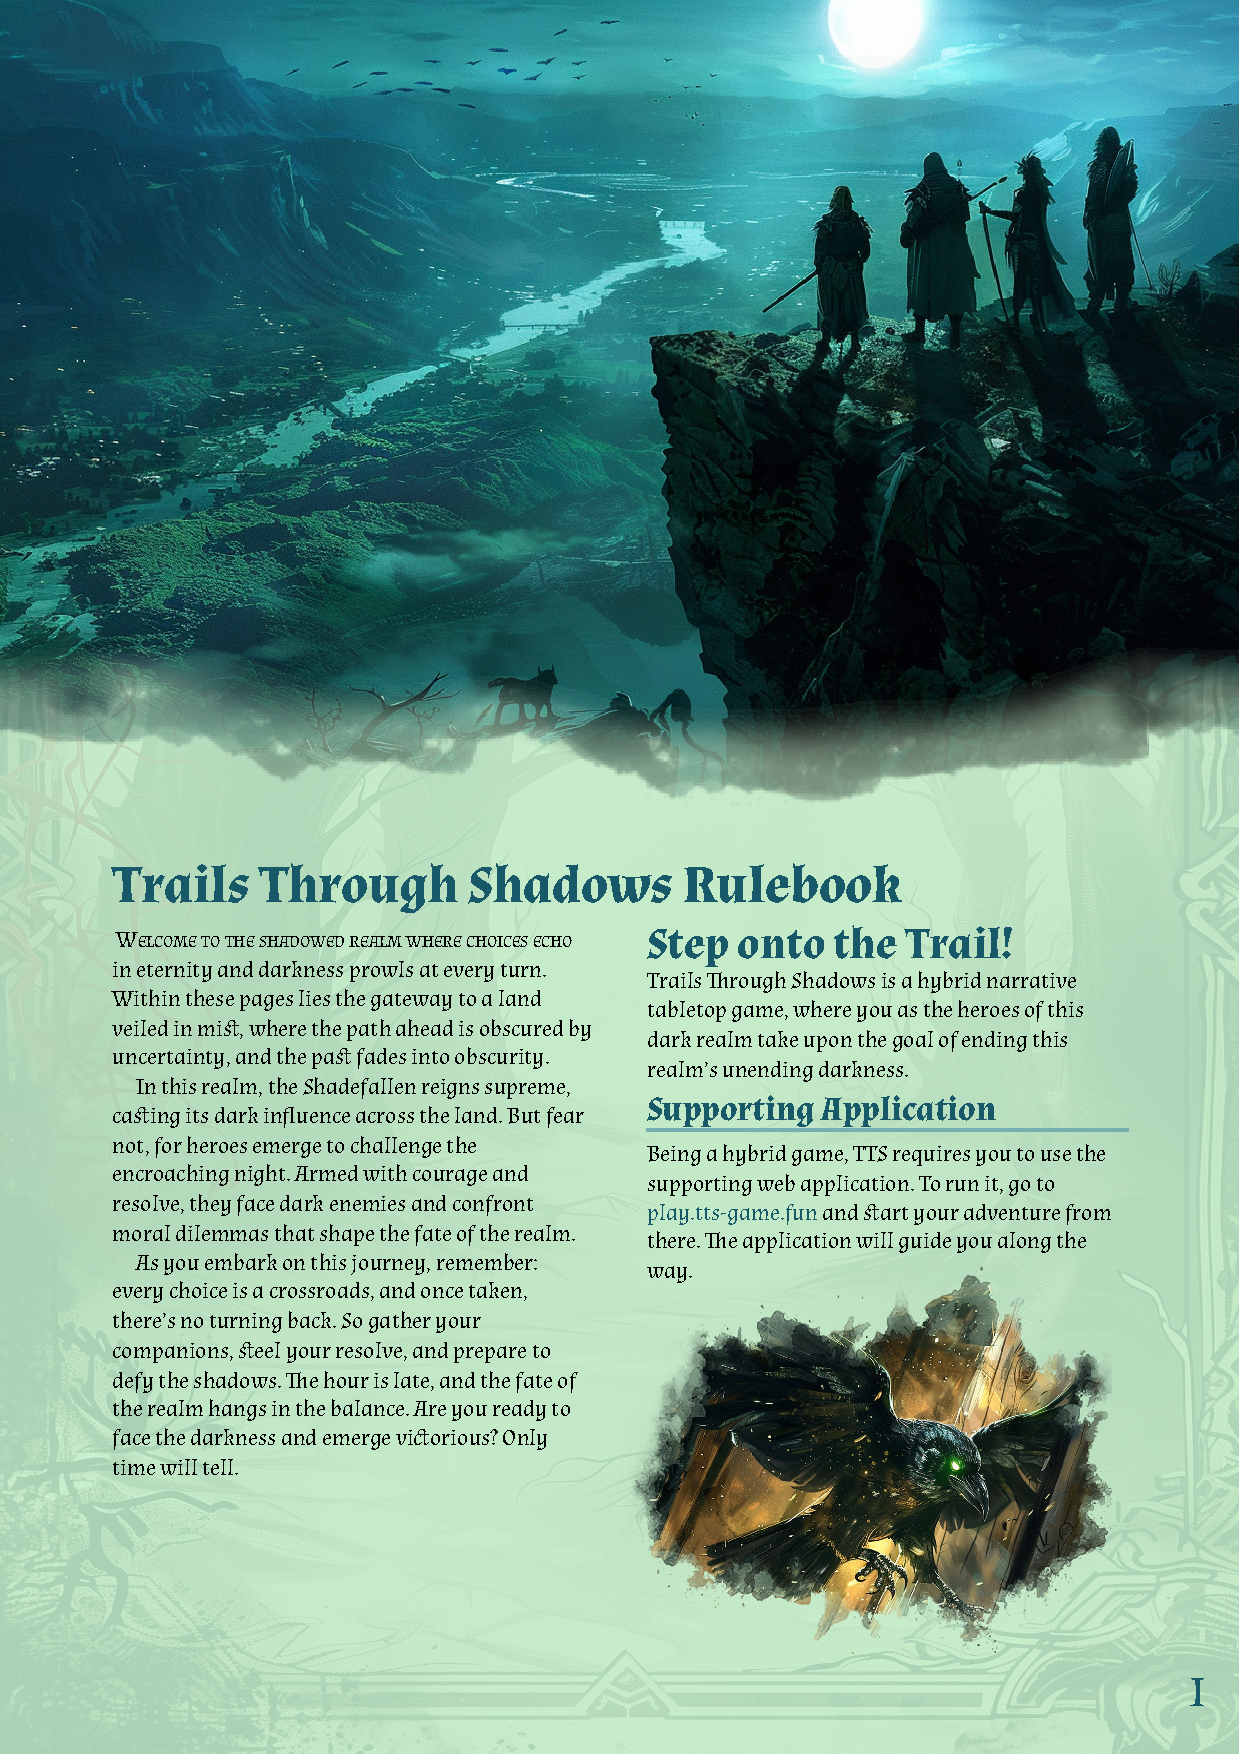
\includegraphics[page=1,height=0.98\textheight]{../../shared/figures/rulebook.pdf}
    \caption{První stránka příručky}
    \label{fig:rulebook1}
\end{figure}

\begin{figure}[h]
    \centering
    \includegraphics[page=2,height=0.98\textheight]{../../shared/figures/rulebook.pdf}
    \caption{Druhá stránka příručky}
    \label{fig:rulebook2}
\end{figure}

\begin{figure}[h]
    \centering
    \includegraphics[page=3,height=0.98\textheight]{../../shared/figures/rulebook.pdf}
    \caption{Třetí stránka příručky}
    \label{fig:rulebook3}
\end{figure}

\begin{figure}[h]
    \centering
    \includegraphics[page=4,height=0.98\textheight]{../../shared/figures/rulebook.pdf}
    \caption{Čtvrtá stránka příručky}
    \label{fig:rulebook4}
\end{figure}
\chapter{Seznam zmíněných stolních her}
\label{sec:GameList}




\end{document}
